\chapter{Analytic \texorpdfstring{\(L\)}{L}-functions}
  Throughout, \(s = \s+it\) and \(u = \tau+ir\) will stand for complex variables with \(\s\), \(\tau\), \(t\), and \(r\) real. We also write
  \[
    (u)_{k} = u(u+1) \cdots (u+(k-1)),
  \]
  for the Pochhammer symbol.
  \section{Analytic Data}
    An \textit{analytic \(L\)-function} \(L(s)\) is a Dirichlet series
    \[
      L(s) = \sum_{n \ge 1}\frac{a_{L}(n)}{n^{s}},
    \]
    with coefficients \(a_{L}(n) \in \C\) such that \(a_{L}(1) = 1\) and satisfying the following properties:
    \begin{enumerate}[align=left]
      \item[\textbf{Analyticity:}] There exists a nonnegative integer \(m_{L}\) such that the Dirichlet series of \(L(s)\) is absolutely convergent for \(\s > 1\) and admits meromorphic continuation to \(\C\) with at most a pole at \(s = 1\) of order \(m_{L}\). Moreover, \((s-1)^{m_{L}}L(s)\) is order \(1\).
      \item[\textbf{Functional Equation:}] There is a positive integer \(q_{L}\), called the \textit{conductor} of \(L(s)\), a positive integer \(d_{L}\) called the \textit{degree} of \(L(s)\), complex numbers \((\mu_{j})_{1 \le j \le d_{L}}\) called the \textit{gamma parameters} of \(L(s)\) that are either real or occur in conjugate pairs and satisfy \(\Re(\mu_{j}) \ge 0\), and a complex number \(\e_{L}\) called the \textit{root number} of \(L(s)\) with \(|\e_{L}| = 1\), all of which determine functions
      \[
        \L(s,L) = q_{L}^{\frac{s}{2}}\g_{L}(s)L(s) \quad \text{and} \quad \g_{L}(s) = \pi^{-\frac{d_{L}s}{2}}\prod_{j}\G\left(\frac{s+\mu_{j}}{2}\right),
      \]
      called the \textit{completion} of \(L(s)\) and the \textit{gamma factor} of \(L(s)\) respectively, satisfying
      \[
        \L(s,L) = \e_{L}\conj{\L(1-\conj{s},L)}.
      \]
      This is called the \textit{functional equation} of \(L(s)\). The tuple \((\e_{L},q_{L},\mu_{1},\ldots,\mu_{d_{L}})\) is called the \textit{functional equation data} of \(L(s)\).
      \item[\textbf{Euler product:}] For every prime \(p\), there exist complex numbers \((\a_{j}(p))_{1 \le j \le d_{L}}\) called the \textit{Euler parameters} of \(L(s)\) at \(p\) satisfying \(|\a_{j}(p)| \le p^{\theta}\) for some \(0 \le \theta < 1\) and are such that \(L(s)\) admits the Euler product
      \[
        L(s) = \prod_{p}(1-\a_{1}(p)p^{-s})^{-1} \cdots (1-\a_{d_{L}}(p)p^{-s})^{-1},
      \]
      for \(\s > 1\). The polynomial \(L_{p}\) defined by
      \[
        L_{p}(T) = (1-\a_{1}(p)T) \cdots (1-\a_{d_{L}}(p)T),
      \]
      is called the \textit{Euler factor} of \(L(s)\) at \(p\). If \(p \nmid q_{L}\) then \(L_{p}\) is of degree \(d_{L}\) while if \(p \mid q_{L}\) then \(L_{p}\) is of degree less than \(d_{L}\).
    \end{enumerate}

    An analytic \(L\)-function is said to be \textit{Selberg class} if it satisfies the following additional property:

    \begin{enumerate}[align=left]
      \item[\textbf{Ramanujan bound:}] We may take \(\theta = 0\) so that \(|\a_{j}(p)| \le 1\).
    \end{enumerate}

    Some comments on the definition of analytic \(L\)-functions are in order.
    \begin{enumerate}[label*=(\roman*)]
      \item As the Dirichlet series of \(L(s)\) converges absolutely for \(\s > 1\) its converges locally absolutely uniformly in this half-plane and therefore defines a holomorphic function there. Moreover, the Euler product necessarily converges locally absolutely uniformly in the same half-plane and hence defines a holomorphic function there as well which agrees with the Dirichlet series.
      \item The bound \(\Re(\mu_{j}) \ge 0\) ensures that the gamma factor is holomorphic in the half-plane \(\s > 0\). As this factor is then guaranteed to be finite and nonzero at \(s = 1\), the completion possesses a pole at \(s = 1\) of order \(r\). By the functional equation, the completion also has a pole at \(s = 0\) of the same order.
      \item If we merely assume \((s-1)^{m_{L}}L(s)\) is finite order then the functional equation forces the order to be \(1\). This can be deduced by considering the entire function
      \[
        s^{m_{L}}(s-1)^{m_{L}}\L(s,L),
      \]
      and applying the Phragm\'en-Lindel\"of convexity principle in vertical strips.
      \item The condition that the root number satisfies \(|\e_{L}| = 1\) isn't strictly necessary. For applying the functional equation twice shows \(|\e_{L}|^{2} = 1\).
      \item As the gamma function is conjugation-equivariant and the gamma parameters are real or occur in conjugate pairs, the gamma factor is also conjugation-equivariant. This means that we can write the functional equation in the form
      \[
        q_{L}^{\frac{s}{2}}\g_{L}(s)L(s) = \e_{L}q_{L}^{\frac{1-s}{2}}\g_{L}(1-s)\conj{L(1-\conj{s})}.
      \]
      \item The Euler product implies that the coefficients \(a_{L}(n)\) are multiplicative and are determined on prime powers by
      \[
        a_{L}(p^{k}) = \sum_{1 \le j_{1} \le \cdots \le j_{k} \le d_{L}}\a_{j_{1}}(p) \cdots \a_{j_{k}}(p).
      \]
      In other words, \(a_{L}(p^{k})\) is the complete symmetric polynomial of degree \(k\) in the Euler parameters at \(p\). If the Ramanujan bound holds, then it follows that \(a_{L}(n) \ll \s_{d_{L}}(n)\). This implies the slightly weaker, but more practical, estimate \(a_{L}(n) \ll_{\e} n^{\e}\).
    \end{enumerate}

    It it clear from the definition that analytic \(L\)-functions are closed under multiplication and that the degree is additive. Moreover, this closure respects Selberg class \(L\)-functions. This makes the set of analytic \(L\)-functions into a graded commutative semigroup where the grading is induced by degree. It follows that there exist irreducible elements with respect to the grading and we say that an analytic \(L\)-function is \textit{primitive} if it such an irreducible. Clearly any analytic \(L\)-function of degree \(1\) is primitive. Moreover, every analytic \(L\)-function factors into a product of primitive \(L\)-functions. Such a factorization is only conjectured to be unique for Selberg class \(L\)-functions. A sufficient condition would be \textit{Selberg's orthogonality conjecture}.

    \begin{conjecture*}[Selberg's orthogonality conjecture]
      For any two primitive Selberg class \(L\)-functions \(L_{1}(s)\) and \(L_{2}(s)\), we have
      \[
        \sum_{p \le x}\frac{a_{L_{1}}(p)\conj{a_{L_{2}}(p)}}{p} = \d_{L_{1},L_{2}}\log\log(x)+O(1).
      \]
    \end{conjecture*}

    Indeed, we have the following result:

    \begin{proposition}
      Assume Selberg's orthogonality conjecture. Then every Selberg class \(L\)-function factors uniquely into a product of primitive Selberg class \(L\)-functions.
    \end{proposition}
    \begin{proof}
      If the factorization into primitive unity \(L\)-functions were not unique, then we would have distinct factorizations satisfying
      \[
        L_{1}(s) \cdots L_{n}(s) = M_{1}(s) \cdots M_{m}(s),
      \]
      for some primitive Selberg class \(L\)-functions \(L_{i}\) and \(M_{j}\). By uniqueness of coefficients of Dirichlet series, compare the \(p\)-th coefficient to see that
      \[
        \sum_{i}a_{L_{i}}(p) = \sum_{j}a_{M_{j}}(p).
      \]
      Now consider
      \[
        \sum_{p < x}\frac{1}{p}\left(\sum_{i}a_{L_{i}}(p)\right)\left(\sum_{j}\conj{a_{M_{j}}(p)}\right) = \sum_{i,j}\sum_{p < x}\frac{a_{L_{i}}(p)\conj{a_{M_{j}}(p)}}{p}.
      \]
      Selberg's orthogonality conjecture implies
      \[
        O(1) = c\log\log(x)+O(1),
      \]
      for some positive integer \(c\) since the factorizations are distinct. This is impossible.
    \end{proof}

    To an analytic \(L\)-function \(L(s)\), we associate its \textit{analytic conductor} \(\mf{q}(s,L)\) defined by
    \[
      \mf{q}(s,L) = q_{L}\mf{q}_{\infty}(s,L),
    \]
    where
    \[
      \mf{q}_{\infty}(s,L) = \prod_{j}(|s+\mu_{j}|+3).
    \]
    The choice of \(3\) in \(|s+\mu_{j}|+3\) is a matter of convenience as could use any positive constant. In particular, it is useful when taking logarithms as \(\log(|s+\mu_{j}|+3) \ge 1\). For legibility, we write also write
    \[
      \mf{q}(L) = \mf{q}(0,L) \quad \text{and} \quad \mf{q}_{\infty}(L) = \mf{q}_{\infty}(0,L).
    \]
    Estimates for the analytic conductor follow from those of the gamma function. Recall from Stirling's formula that
    \begin{equation}\label{equ:vertical_strip_gamma_estimates}
      \G(s) \ll_{\e} (|t|+3)^{\s-\frac{1}{2}}e^{-\frac{\pi}{2}|t|} \quad \text{and} \quad \frac{1}{\G(s)} \ll (|t|+3)^{\frac{1}{2}-\s}e^{\frac{\pi}{2}|t|},
    \end{equation}
    for bounded \(\s\) provided that in the former estimate \(s\) is at least distance \(\e\) away from the poles of the gamma function. Hence
    \[
      \frac{\G(1-s)}{\G(s)} \ll_{\e} (|t|+3)^{1-2\s},
    \]
    for bounded \(\s\) provided \(s\) is at least distance \(\e\) away from the poles of \(\G(1-s)\). Then the estimates
     \begin{equation}\label{equ:gamma_factor_analytic_conductor_estimate}
      \frac{\g_{L}(1-s)}{\g_{L}(s)} \ll_{\e} \mf{q}_{\infty}(s,L)^{\frac{1}{2}-\s} \quad \text{and} \quad q_{L}^{\frac{1}{2}-s}\frac{\g_{L}(1-s)}{\g_{L}(s)} \ll_{\e} \mf{q}(s,L)^{\frac{1}{2}-\s},
    \end{equation}
    hold for bounded \(\s\) provided \(s\) is at least distance \(\e\) away from the poles of \(\g_{L}(1-s)\). An associated estimate can be obtain for the logarithmic derivative of the analytic conductor. Recall from the logarithm of Stirling's formula that
    \[
      \frac{\G'}{\G}(s) \ll \log(|s|+3),
    \]
    provided \(\s\) is bounded and \(s\) is at least distance \(\e\) away from the poles of the gamma function. Then the estimates
    \begin{equation}\label{equ:digamma_gamma_factor_analytic_conductor_estimate}
      \frac{\g_{L}'}{\g_{L}}(s) \ll_{\e} \log\mf{q}_{\infty}(s,L) \quad \text{and} \quad \log{q_{L}}+\frac{\g_{L}'}{\g_{L}}(s) \ll_{\e} \log\mf{q}(s,L),
    \end{equation}
    hold for bounded \(\s\) provided \(s\) is at least distance \(\e\) away from the poles of the gamma factor.
    
    The \textit{critical strip} of an analytic \(L\)-function is the vertical strip left invariant by the transformation \(s \mapsto 1-s\). This region can also be described as
    \[
      \left\{s \in \C:\left|\s-\frac{1}{2}\right| \le \frac{1}{2}\right\}.
    \]

    \begin{figure}[ht]
      \centering
      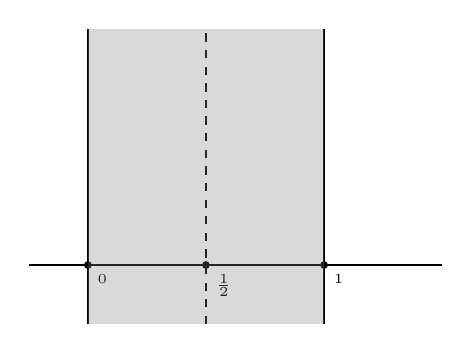
\begin{tikzpicture}[scale=1.5]
        \def\xmin{-0.5} \def\xmax{3}
        \def\ymin{-0.5} \def\ymax{2}
        \draw[thick] (\xmin,0) -- (\xmax,0);
        \draw[thick] (0,\ymin) -- (0,\ymax);
        \draw[thick] (2,\ymin) -- (2,\ymax);
        \draw[dashed] (1,\ymin) -- (1,\ymax);

        \node at (0,0) [below right] {\tiny{\(0\)}};
        \node at (0,0) [circle,fill,inner sep=1pt]{};
        \node at (1,0) [below right] {\tiny{\(\frac{1}{2}\)}};
        \node at (1,0) [circle,fill,inner sep=1pt]{};
        \node at (2,0) [below right] {\tiny{\(1\)}};
        \node at (2,0) [circle,fill,inner sep=1pt]{};

        \begin{scope}
          \path[clip] (0,\ymin) -- (0,\ymax) -- (2,\ymax) -- (2,\ymin) -- cycle;
          \fill[gray,opacity=0.3] (0,\ymin) rectangle (2,\ymax);
        \end{scope}
      \end{tikzpicture}
      \caption{The critical strip.}
      \label{fig:critical_strip}
    \end{figure}

    The \textit{critical line} is the vertical line left invariant by the transformation \(s \mapsto 1-s\) which is also given by \(\s = \frac{1}{2}\). The critical line bisects the critical strip vertically. The \textit{central point} is the fixed point of the transformation \(s \mapsto 1-s\), in other words, the point \(s = \frac{1}{2}\). Clearly the central point is also the center of the critical line. The critical strip, critical line, and central point are all displayed in \cref{fig:critical_strip}.

    In the half-plane \(\s > 1\) we may study the analytic properties of \(L(s)\) via its Dirichlet series. Using the functional equation, we may write
    \[
      L(s) = \e_{L}q_{L}^{\frac{1}{2}-s}\frac{\g_{L}(1-s)}{\g_{L}(s)}\conj{L(1-\conj{s})}.
    \]
    This permits the study of \(L(s)\) in the half-plane \(\s < 0\) by using the Dirichlet series of \(\conj{L(1-\conj{s})}\) and the the functional equation data. The interior of the critical strip is exactly the region where we cannot use either of these methods to study the analytic properties of \(L(s)\). Of course, anything may be possible on the boundary lines \(\s = 0\) and \(\s = 1\) (for example Landau's theorem).
  \section{The Approximate Functional Equation}
    Despite not being able to study an analytic \(L\)-function \(L(s)\) in the critical strip by means of Dirichlet series, there is formula which acts as a compromise between the functional equation and the Dirichlet series. This formula is known as the approximate functional equation. The usefulness comes from the fact that the approximate functional equation is valid inside of the critical strip and therefore can be used to obtain analytic properties about \(L(s)\) in that region. We will first derive a preliminary result showing \(L(s)\) has at most polynomial growth.

    \begin{proposition}\label{prop:L_function_bounded_in_vertical_strips}
      Let \(L(s)\) be an analytic \(L\)-function with \(\s\) bounded and \(\s\) at least distance \(\e\) away from the possible pole at \(s = 1\). Then there is a positive constant \(A\) such that
      \[
        L(s) \ll_{\e} (|t|+3)^{A}.
      \]
    \end{proposition}
    \begin{proof}
      Observe that \((s-1)^{m_{L}}L(s) \ll_{\e} (|t|+3)^{m_{L}}\) on the vertical line \(\s = \max(1+\e,\s_{2})\). Now suppose \(\s = \min(-\e,\s_{1})\). On this vertical line, the functional equation and \cref{equ:gamma_factor_analytic_conductor_estimate} together show
      \[
        L(s) \ll_{\e} \mf{q}(s,L)^{\frac{1}{2}-\s}\conj{L(1-\conj{s})}.
      \]
      Hence there exists a positive constant \(A''\) with
      \[
        (s-1)^{m_{L}}L(s) \ll_{\e} (|t|+3)^{A''},
      \]
      on the vertical line \(\s = \min(-\e,\s_{1})\). As \((s-1)^{m_{L}}L(s)\) is entire and of order \(1\), we can apply the Phragm\'en-Lindel\"of convexity principle to \((s-1)^{m_{L}}L(s)\) the vertical strip \(\min(-\e,\s_{1}) \le \s \le \max(1+\e,\s_{2})\). Whence there is a positive constant \(A'\) such that
      \[
        (s-1)^{m_{L}}L(s) \ll_{\e} (|t|+3)^{A'},
      \]
      provided \(\s\) is bounded. Assuming \(s\) is at least distance \(\e\) away from the possible pole at \(s = 1\), diving by \((s-1)^{m_{L}}\) completes the proof.
    \end{proof}

    We are almost ready to prove the approximate function equation for an analytic \(L\)-function \(L(s)\). The formula itself consists of two sums representing the Dirichlet series at \(s\) and a dualized Dirichlet series at \(1-s\) as well as a potential residue term. The dual sum comes equip with a term containing the data of the functional equation. Both sums will also be dampened by a smooth cutoff function. In the statement of the approximate function equation, we will make use of a test function \(\Phi(u)\). We require \(\Phi(u)\) be an even holomorphic function bounded in the vertical strip \(|\tau| < a+1\) for some \(a > 1\) and such that \(\Phi(0) = 1\). For \(s\) in the critical strip, we let \(V_{s}(y)\) be the inverse Mellin transform
    \[
      V_{s}(y) = \frac{1}{2\pi i}\int_{(a)}\frac{\g_{L}(s+u)}{\g_{L}(s)}\Phi(u)y^{-u}\frac{du}{u},
    \]
    defined for \(y > 0\). Stirling's formula implies
    \[
      \frac{\G(s+u)}{\G(s)} \ll_{\e} \frac{(|t+r|+3)^{\s+\tau-\frac{1}{2}}}{(|t|+3)^{\s-\frac{1}{2}}}e^{-\frac{\pi}{2}(|t+r|-|t|)},
    \]
    for \(s\) in the critical strip and bounded \(\tau\) provided \(s+u\) is at least distance \(\e\) away from the poles of the gamma function. Whence
    \begin{equation}\label{equ:gamma_factor_s_and_u_estimate}
      \frac{\g_{L}(s+u)}{\g_{L}(s)} \ll_{\e} \frac{\mf{q}_{\infty}(s+u)^{\frac{\s+\tau}{2}-\frac{1}{4}}}{\mf{q}_{\infty}(s)^{\frac{\s}{2}-\frac{1}{4}}}e^{-d_{L}\frac{\pi}{2}(|t+r|-|t|)},
    \end{equation}
    for \(s\) in the critical strip and bounded \(\tau\) provided \(s+u\) is at least distance \(\e\) away from the poles of the gamma factor. Since \(\Phi(u)\) is bounded in the vertical strip \(|\tau| < a+1\), the integrand exhibits exponential decay. Therefore the integral is locally absolutely uniformly bounded and hence \(V_{s}(y)\) is smooth. The function \(V_{s}(y)\) is the smooth cutoff function mentioned previously. We will also let \(\e_{L}(s)\) be given by
    \[
      \e_{L}(s) = \e_{L}q_{L}^{\frac{1}{2}-s}\frac{\g_{L}(1-s)}{\g_{L}(s)}.
    \]
    This term appears as a factor in the dual sum accounting for the functional equation data. We now prove the \textit{approximate function equation}:

    \begin{theorem*}[Approximate functional equation]
      Suppose \(L(s)\) is an analytic \(L\)-function, \(\Phi(u)\) is an even holomorphic function bounded in the vertical strip \(|\tau| < a+1\) for some \(a > 1\) and such that \(\Phi(0) = 1\), and let \(X > 0\). Then for \(s\) in the critical strip, we have
      \[
        L(s) = \sum_{n \ge 1}\frac{a_{L}(n)}{n^{s}}V_{s}\left(\frac{n}{\sqrt{q_{L}}X}\right)+\e_{L}(s)\sum_{n \ge 1}\frac{\conj{a_{L}(n)}}{n^{1-s}}V_{1-s}\left(\frac{nX}{\sqrt{q_{L}}}\right)+\frac{R(s,X,L)}{q_{L}^{\frac{s}{2}}\g_{L}(s)},
      \]
      where \(R(s,X,L)\) is given by
      \[
        R(s,X,L) = \Res_{u = 1-s}\frac{\L(s+u,L)\Phi(u)X^{u}}{u}+\Res_{u = -s}\frac{\L(s+u,L)\Phi(u)X^{u}}{u}.
      \]
    \end{theorem*}
    \begin{proof}
      Consider the integral
      \[
        \frac{1}{2\pi i}\int_{(a)}\L(s+u,L)\Phi(u)X^{u}\,\frac{du}{u}.
      \]    
      Stirling's formula shows that \(\g_{L}(s+u)\) exhibits exponential decay while \(L(s+u)\) has at most polynomial growth by \cref{prop:L_function_bounded_in_vertical_strips}. Since \(\Phi(u)\) is bounded in the vertical strip \(|\tau| < a+1\), it follows that the integrand exhibits exponential decay. Therefore the integral is locally absolutely uniformly bounded. We will evaluate the integral in two ways. On the one hand, we can expand \(L(s+u)\) inside the integrand as a Dirichlet series and by absolute boundedness of the integral we may interchange the sum and integral. A short computation shows that this is
      \[
        q_{L}^{\frac{s}{2}}\g_{L}(s)\sum_{n \ge 1}\frac{a_{L}(n)}{n^{s}}V_{s}\left(\frac{n}{\sqrt{q_{L}}X}\right).
      \]
      On the other hand, we can shift the line of integration to \((-a)\). In doing so we pass by a simple pole at \(u = 0\) and possible poles at \(u = 1-s\) and \(u = -s\) giving
      \[
        \frac{1}{2\pi i}\int_{(-a)}\L(s+u,L)\Phi(u)X^{u}\,\frac{du}{u}+\L(s,L)+R(s,X,L).
      \]
      Apply the functional equation and perform the change of variables \(u \mapsto -u\) to rewrite this as
      \[
        -\e_{L}\frac{1}{2\pi i}\int_{(a)}\conj{\L(1-\conj{s+u},L)}\Phi(u)X^{-u}\,\frac{du}{u}+\L(s,L)+R(s,X,L).
      \]
      Analogous to the above, we can now expand \(\conj{L(1-\conj{s+u})}\) inside the integrand as a Dirichlet series and by absolute boundedness of the integral we may interchange the sum and integral. A short computation shows that our previous expression becomes
      \[
        -\e_{L}q_{L}^{\frac{1-s}{2}}\g_{L}(1-s)\sum_{n \ge 1}\frac{\conj{a_{L}(n)}}{n^{1-s}}V_{s}\left(\frac{nX}{\sqrt{q_{L}}}\right)+\L(s,L)+R(s,X,L).
      \]
      Equating these two evaluations and isolating the completion gives
      \begin{align*}
        \L(s,L) &= q_{L}^{\frac{s}{2}}\g_{L}(s)\sum_{n \ge 1}\frac{a_{L}(n)}{n^{s}}V_{s}\left(\frac{n}{\sqrt{q_{L}}X}\right) \\
        &+ \e_{L}q_{L}^{\frac{1-s}{2}}\g_{L}(1-s)\sum_{n \ge 1}\frac{\conj{a_{L}(n)}}{n^{1-s}}V_{1-s}\left(\frac{nX}{\sqrt{q_{L}}}\right)+R(s,X,L).
      \end{align*}
      Diving by \(q_{L}^{\frac{s}{2}}\g_{L}(s)\) completes the proof.
    \end{proof}

    Let us now show how \(V_{s}(y)\) has the effect of dampening the two dual sums appearing on the right-hand side of the approximate functional equation. In practice, it is common to choose \(\Phi(u)\) such that it has exponential decay and we can make the vertical strip on which it is bounded arbitrarily wide. For example, let
    \[
      \Phi(u) = \cos^{-4d_{L}M}\left(\frac{\pi u}{4M}\right),
    \]
    for some positive integer \(M\). Clearly \(\Phi(u)\) is an even holomorphic function in the vertical strip \(|\tau| < (2M-1)+1\) and satisfies \(\Phi(0) = 1\). In view of the identity \(\cos(u) = \frac{e^{iu}+e^{-iu}}{2}\), we find that
    \begin{equation}\label{equ:choice_for_V_decay_estimate}
     \cos^{-4d_{L}M}\left(\frac{\pi u}{4M}\right) \ll_{\e} e^{-d_{L}\pi|r|},
    \end{equation}
    for \(|\tau| < (2M-1)+1\) provided \(u\) is at least distance \(\e\) away from the poles of \(\Phi(u)\). Therefore \(\Phi(u)\) admits exponential decay. For this choice of \(\Phi(u)\), \(V_{s}(y)\) and its derivatives will possess rapid decay.

    \begin{proposition}\label{prop:V_function_decay}
      Let \(L(s)\) be an analytic \(L\)-function, set \(\Phi(u) = \cos^{-4d_{L}M}\left(\frac{\pi u}{4M}\right)\) for some positive integer \(M\), and let \(V_{s}(y)\) be the inverse Mellin transform defined by
      \[
        V_{s}(y) = \frac{1}{2\pi i}\int_{(2M-1)}\frac{\g_{L}(s+u)}{\g_{L}(s)}\Phi(u)y^{-u}\frac{du}{u}.
      \]
      Then for \(s\) in the critical strip, any nonnegative integer \(k\), and positive integer \(N\) with \(N < 2M\), \(V_{s}(y)\) satisfies the estimates
      \[
        (-y)^{k}V_{s}^{(k)}(y) = \begin{cases} \d_{k,0}+O_{\e}\left(\left(\frac{y}{\sqrt{\mf{q}_{\infty}(s,L)}}\right)^{N}\right) & \text{if \(y \ll \sqrt{\mf{q}_{\infty}(s,L)}\)}, \\ O_{\e}\left(\left(\frac{y}{\sqrt{\mf{q}_{\infty}(s,L)}}\right)^{-N}\right) & \text{if \(y \gg \sqrt{\mf{q}_{\infty}(s,L)}\)}. \end{cases}
      \]
      In particular,
      \[
        (-y)^{k}V_{s}^{(k)}(y) \ll_{\e} \left(1+\frac{y}{\sqrt{\mf{q}_{\infty}(s,L)}}\right)^{-N}.
      \]
    \end{proposition}
    \begin{proof}
      As we have already seen, the integrand defining \(V_{s}(y)\) admits exponential decay. This permits us to differentiate under the integral sign and shift the line of integration. The former shows
      \[
        (-y)^{k}V_{s}^{(k)}(y) = \frac{1}{2\pi i}\int_{(2M-1)}\frac{\g_{L}(s+u)}{\g_{L}(s)}\Phi(u)(u)_{k}y^{-u}\frac{du}{u}.
      \]
      Shifting to \((-N)\), we pass by a simple pole at \(u = 0\) of residue \(1\) if and only if \(k = 0\). This gives
      \[
        (-y)^{k}V_{s}^{(k)}(y) = \d_{k,0}+\frac{1}{2\pi i}\int_{(-N)}\frac{\g_{L}(s+u)}{\g_{L}(s)}\Phi(u)(u)_{k}y^{-u}\frac{du}{u}.
      \]
      This integrand also exhibits exponential decay since the Pochhammer symbol grows polynomially. Therefore the integral is dominated by the contribution when \(u \ll 1\) and the \cref{equ:gamma_factor_s_and_u_estimate,equ:choice_for_V_decay_estimate} together show
      \[
        (-y)^{k}V_{s}^{(k)}(y) = \d_{k,0}+O_{\e}\left(\left(\frac{y}{\sqrt{\mf{q}_{\infty}(s,L)}}\right)^{N}\right).
      \]
      If we instead shift to \((N)\), we do not pass by any poles and obtain
      \[
        (-y)^{k}V_{s}^{(k)}(y) = \frac{1}{2\pi i}\int_{(N)}\frac{\g_{L}(s+u)}{\g_{L}(s)}\Phi(u)(u)_{k}y^{-u}\frac{du}{u}.
      \]
      An analogous argument to estimate the remaining integral shows
      \[
        (-y)^{k}V_{s}^{(k)}(y) = O_{\e}\left(\left(\frac{y}{\sqrt{\mf{q}_{\infty}(s,L)}}\right)^{-N}\right).
      \]
      From these \(O\)-estimates we obtain nontrivial bounds in the ranges \(y \ll \sqrt{\mf{q}_{\infty}(s,L)}\) and \(y \gg \sqrt{\mf{q}_{\infty}(s,L)}\) respectively. Combining both of these estimates produces the bound
      \[
        (-y)^{k}V_{s}^{(k)}(y) \ll_{\e} \left(1+\frac{y}{\sqrt{\mf{q}_{\infty}(s,L)}}\right)^{-N}.
      \]
    \end{proof}

    With our choice of \(\Phi(u)\), this result shows that \(V_{s}(y)\) is essentially \(1\) up to some admissible error for \(y \ll \sqrt{\mf{q}_{\infty}(s,L)}\) and exhibits rapid decay thereafter as we can take \(M\) (and hence \(N\)) to be arbitrarily large.
    
    In a similar spirit to the approximate functional equation, a useful summation formula can be derived from the functional equation. Let \(\psi(y)\) be a smooth weight where \(\Psi(s)\) is its Mellin transform. Then we will let \(\psi(y,L)\) be the inverse Mellin transform
    \[
      \psi(y,L) = \frac{1}{2\pi i}\int_{(a)}q_{L}^{s}\frac{\g_{L}(s)}{\g_{L}(1-s)}y^{-s}\Psi(1-s)\,ds,
    \]
    defined for \(y > 0\) where \(a > 1\). By our choice of \(\psi(y)\), its inverse Mellin transform \(\Psi(s)\) has rapid decay. Since \(L(s)\) has at most polynomial growth by \cref{prop:L_function_bounded_in_vertical_strips}, the integrand has rapid decay as well. Therefore the integral is locally absolutely uniformly bounded and hence \(\psi(y,L)\) is smooth for \(y > 0\). Our result is the following:


    \begin{theorem}
      Let \(L(s)\) be an analytic \(L\)-function and let \(\psi(y)\) be a smooth weight where \(\Psi(s)\) is its Mellin transform. Then
      \[
        \sum_{n \ge 1}a_{L}(n)\psi(n) = \frac{\e_{L}}{\sqrt{q_{L}}}\sum_{n \ge 1}\conj{a_{L}(n)}\psi(n,L)+R(L)\Psi(1),
      \]
      where \(R(L)\) is given by
      \[
        R(L) = \Res_{s = 1}L(s).
      \]
    \end{theorem}
    \begin{proof}
      Smoothed Perron's formula implies
      \[
        \sum_{n \ge 1}a_{L}(n)\psi(n) = \frac{1}{2\pi i}\int_{(a)}L(s)\Psi(s)\,ds.
      \]
      By our choice of \(\psi(y)\), its inverse Mellin transform \(\Psi(s)\) has rapid decay. Since \(L(s)\) has at most polynomial growth by \cref{prop:L_function_bounded_in_vertical_strips}, the integrand has rapid decay as well. Therefore the integral is locally absolutely uniformly bounded which permits us to shift the line of integration. Shifting to \((1-a)\), we pass by a potential pole at \(s = 1\) and obtain
      \[
        \sum_{n \ge 1}a_{L}(n)\psi(n) = \frac{1}{2\pi i}\int_{(1-a)}L(s)\Psi(s)\,ds+R(L)\Psi(1).
      \]
      Apply the functional equation to rewrite this equality in the form
      \[
        \sum_{n \ge 1}a_{L}(n)\psi(n) = \frac{1}{2\pi i}\int_{(1-a)}\e_{L}q_{L}^{\frac{1}{2}-s}\frac{\g_{L}(1-s)}{\g_{L}(s)}\conj{L(1-\conj{s})}\Psi(s)\,ds+R(L)\Psi(1).
      \]
      Performing the change of variables \(s \mapsto 1-s\) in this latter integral gives
      \[
        \sum_{n \ge 1}a_{L}(n)\psi(n) = \frac{1}{2\pi i}\int_{(a)}\e_{L}q_{L}^{s-\frac{1}{2}}\frac{\g_{L}(s)}{\g_{L}(1-s)}\conj{L(\conj{s})}\Psi(1-s)\,ds+R(L)\Psi(1).
      \]
      The proof is complete upon expanding \(\conj{L(\conj{s})}\) as a Dirichlet series, interchanging the sum and integral by absolute boundedness of the integral, and factoring out \(\frac{\e_{L}}{\sqrt{q_{L}}}\).
    \end{proof}
  \section{The Riemann Hypothesis and Nontrivial Zeros}
    The zeros of an \(L\)-functions \(L(s)\) has interesting behavior. From the Euler product we immediately see that \(L(s)\) has no zeros in the half-plane \(\s > 1\). We can use the functional equation to determine the zeros for \(\s < 0\). Indeed, write the functional equation in the form
    \[
      L(s) = \e_{L}q_{L}^{\frac{1}{2}-s}\frac{\g_{L}(1-s)}{\g_{L}(s)}\conj{L(1-\conj{s})}.
    \] 
    So for \(\s < 0\), we see that \(\conj{L(1-\conj{s})}\) is nonzero. Moreover, \(\g_{L}(1-s)\) is as well. Together this means that for \(\s < 0\) the poles of \(\g_{L}(s)\) are zeros of \(L(s)\). Such a zero is called a \textit{trivial zero} of \(L(s)\). From the definition of the gamma factor, they are all simple and of the form \(s = -(\mu_{j}+2n)\) for some gamma parameter \(\mu_{j}\) and some nonnegative integer \(n\).
    
    Any other zero of \(L(s)\) is called a \textit{nontrivial zero} and it necessarily lies inside of the critical strip. Let \(\rho\) be a nontrivial zero of \(L(s)\). Then the functional equation implies that \(1-\conj{\rho}\) is also a nontrivial zero of \(L(s)\). This means that nontrivial zeros occur in pairs
    \[
      \rho \quad \text{and} \quad 1-\conj{\rho}.
    \]
    It is possible to say more when \(L(s)\) takes real values for \(s > 1\). For in this case, the Schwarz reflection principle implies \(L(\conj{s}) = \conj{L(s)}\) and that \(L(s)\) takes real values on the entire real axis save for the possible pole at \(s = 1\). It follows from the functional equation that \(\conj{\rho}\) and \(1-\rho\) are also nontrivial zeros. Therefore the nontrivial zeros of \(L(s)\) come in sets of four
    \[
      \rho, \quad \conj{\rho}, \quad 1-\rho, \quad \text{and} \quad 1-\conj{\rho}.
    \]
    See \cref{fig:symmetric_nontrivial_zeros} for an example of this symmetry.

    \begin{figure}[ht]
      \centering
      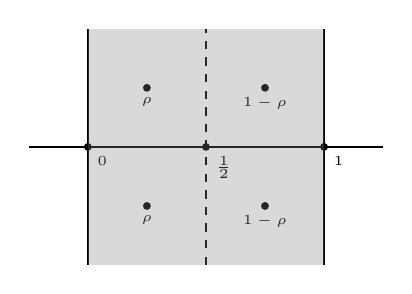
\begin{tikzpicture}[scale=1.5]
        \def\xmin{-0.5} \def\xmax{2.5}
        \def\ymin{-1} \def\ymax{1}
        \draw[thick] (\xmin,0) -- (\xmax,0);
        \draw[thick] (0,\ymin) -- (0,\ymax);
        \draw[thick] (2,\ymin) -- (2,\ymax);
        \draw[dashed] (1,\ymin) -- (1,\ymax);

        \node at (1.5,0.5) [circle,fill,inner sep=1pt]{};
        \node at (1.5,0.5) [below] {\tiny{\(1-\conj{\rho}\)}};
        \node at (0.5,0.5) [circle,fill,inner sep=1pt]{};
        \node at (0.5,0.5) [below] {\tiny{\(\rho\)}};
        \node at (1.5,-0.5) [circle,fill,inner sep=1pt]{};
        \node at (1.5,-0.5) [below] {\tiny{\(1-\rho\)}};
        \node at (0.5,-0.5) [circle,fill,inner sep=1pt]{};
        \node at (0.5,-0.5) [below] {\tiny{\(\conj{\rho}\)}};

        \node at (0,0) [below right] {\tiny{\(0\)}};
        \node at (0,0) [circle,fill,inner sep=1pt]{};
        \node at (1,0) [below right] {\tiny{\(\frac{1}{2}\)}};
        \node at (1,0) [circle,fill,inner sep=1pt]{};
        \node at (2,0) [below right] {\tiny{\(1\)}};
        \node at (2,0) [circle,fill,inner sep=1pt]{};

        \begin{scope}
          \path[clip] (0,\ymin) -- (0,\ymax) -- (2,\ymax) -- (2,\ymin) -- cycle;
          \fill[gray,opacity=0.3] (0,\ymin) rectangle (2,\ymax);
        \end{scope}
        \end{tikzpicture}
      \caption{Symmetric nontrivial zeros.}
      \label{fig:symmetric_nontrivial_zeros}
    \end{figure}

    The \textit{Riemann hypothesis} for \(L(s)\) says that this symmetry should be as simple as possible.

    \begin{conjecture*}[Riemann hypothesis, \(L(s)\)]
      The nontrivial zeros of the analytic \(L\)-function \(L(s)\) all lie on the vertical line \(\s = \frac{1}{2}\).
    \end{conjecture*}

    While stated as a conjecture, we not expect the Riemann hypothesis to hold for just any analytic \(L\)-function. We do however expect it to hold for Selberg class \(L\)-functions. In particular, the \textit{Selberg class Riemann hypothesis} says that this symmetry should hold for any Selberg class \(L\)-function:

    \begin{conjecture*}[Selberg class Riemann hypothesis]
      The nontrivial zeros of any Selberg class \(L\)-function \(L(s)\) lie on the vertical line \(\s = \frac{1}{2}\).
    \end{conjecture*}

    So far, the Riemann hypothesis remains completely out of reach for any analytic \(L\)-function and thus the Selberg class Riemann hypothesis does as well.
  \section{The Lindel\"of Hypothesis and Estimates on the Critical Line}
    Instead of asking about the zeros of an analytic \(L\)-function \(L(s)\) on the critical line we can ask about its growth there. Let us begin this investigation by deriving an upper bound for \(L(s)\) on the critical line using the Phragm\'en-Lindel\"of convexity principle. This amounts to a more refined version of the argument used in \cref{prop:L_function_bounded_in_vertical_strips} for the critical strip.

    \begin{theorem}\label{thm:convexity_bound_for_L_function_in_critial_strip}
      Let \(L(s)\) be an analytic \(L\)-function. Then for \(-\e \le \s \le 1+\e\), we have
      \[
        L(s) \ll_{\e} \mf{q}(s,L)^{\frac{1-\s}{2}+\e},
      \]
      provided \(s\) is at least distance \(\e\) away from the possible pole at \(s = 1\).
    \end{theorem}
    \begin{proof}
      Since \((s-1)^{r_{L}}L(s)\) is entire and of order \(1\), we will apply the Phragm\'en-Lindel\"of convexity principle just outside the edges of the critical strip. Just past the right edge along the vertical line \(\s = 1+\e\), we have
      \[
        (s-1)^{r_{L}}L(s) \ll_{\e} (s-1)^{r_{L}}.
      \]
      Just past the left edge along the vertical line \(\s = -\e\), the functional equation and \cref{equ:gamma_factor_analytic_conductor_estimate} together imply the bound
      \[
        (s-1)^{r_{L}}L(s) \ll_{\e} (s-1)^{r_{L}}\mf{q}(s,L)^{\frac{1}{2}+\e}.
      \]
      By the Phragm\'en-Lindel\"of convexity principle, we obtain
      \[
        (s-1)^{r_{L}}L(s) \ll_{\e} (s-1)^{r_{L}}\mf{q}(s,L)^{\frac{1-\s}{2}+\e},
      \]
      provided \(-\e \le \s \le 1+\e\). Assuming \(s\) is at least distance \(\e\) away from the possible pole at \(s = 1\), dividing by \((s-1)^{r_{L}}\) completes the proof.
    \end{proof}
    
    At the critical line this theorem produces the bound
    \[
      L\left(\frac{1}{2}+it\right) \ll_{\e} \mf{q}\left(\frac{1}{2}+it,L\right)^{\frac{1}{4}+\e}.
    \]
    This is known as the \textit{convexity bound} for \(L(s)\). The \textit{Lindel\"of hypothesis} for \(L(s)\) says that the exponent can be reduced to \(\e\):

    \begin{conjecture*}[Lindel\"of hypothesis, \(L(s)\)]
      The analytic \(L\)-function \(L(s)\) satisfies
      \[
        L\left(\frac{1}{2}+it\right) \ll_{\e} \mf{q}\left(\frac{1}{2}+it,L\right)^{\e}.
      \]
    \end{conjecture*}

    Unlike the Riemann hypothesis, the Lindel\"of hypothesis is expected to hold for any analytic \(L\)-function. In any case, the \textit{Selberg class Lindel\"of hypothesis} says that the exponent can be reduced to \(\e\) for any Selberg class \(L\)-function:

    \begin{conjecture*}[Selberg class Lindel\"of hypothesis]
      Any Selberg class \(L\)-function \(L(s)\) satisfies
      \[
        L\left(\frac{1}{2}+it\right) \ll_{\e} \mf{q}\left(\frac{1}{2}+it,L\right)^{\e}.
      \]
    \end{conjecture*}

    Like the Riemann hypothesis, we have been unable to prove the Lindel\"of hypothesis for any analytic \(L\)-function. However, in practice the Lindel\"of hypothesis is more tractable. Generally speaking, any improvement upon the exponent in the convexity bound in any aspect of the analytic conductor is called a \textit{subconvexity estimate} (or a \textit{convexity breaking bound}). In the uniform case, we would like to prove bounds of the form
    \[
      L\left(\frac{1}{2}+it\right) \ll_{\e} \mf{q}\left(\frac{1}{2}+it,L\right)^{\d+\e},
    \]
    for some \(0 \le \d \le \frac{1}{4}\). The convexity bound says that we may take \(\d = \frac{1}{4}\) while the Lindel\"of hypothesis for \(L(s)\) implies that we may take \(\d = 0\). Any uniform subconvexity estimate would give a \(\d\) strictly less than \(\frac{1}{4}\). Subconvexity estimates are viewed with great interest. This is primarily because of their connection to the Lindel\"of hypothesis, but also because any improvement upon the convexity bound in any aspect of the analytic conductor often has drastic consequences in applications.

    \begin{remark}
      Some subconvexity bounds are deserving of names. The cases \(\d = \frac{3}{16}\) and \(\d = \frac{1}{6}\) are referred to as the \textit{Burgess bound} and \textit{Weyl bound} respectively.
    \end{remark}
    
    With a little more work, we can obtain a a similar bound for the derivatives of analytic \(L\)-functions. First observe that \cref{thm:convexity_bound_for_L_function_in_critial_strip} gives the estimate
    \[
      L(s) \ll_{\e} \mf{q}\left(\frac{1}{2}+it,L\right)^{\frac{1}{4}+\e},
    \]
    in the vertical strip \(\left|\s-\frac{1}{2}\right| \le \frac{\e}{2}\). This is just slightly stronger than the convexity bound. By Cauchy's integral formula, we may write
    \[
      L^{(k)}\left(\frac{1}{2}+it\right) = \frac{k!}{2\pi i}\int_{\eta}\frac{L(s)}{(s-\frac{1}{2}-it)^{k+1}}\,ds,
    \]
    where \(\eta\) is the circle about \(\frac{1}{2}+it\) of radius \(\frac{\e}{2}\). The parameterization \(u \mapsto \frac{1}{2}+it+\frac{\e}{2}e^{i\t}\) for \(\eta\) shows that
    \[
      L^{(k)}\left(\frac{1}{2}+it\right) \ll_{\e} \mf{q}\left(\frac{1}{2}+it,L\right)^{\frac{1}{4}+\e}.
    \]
    This is known as the \textit{convexity bound} for \(L^{(k)}(s)\).

    We now turn to the question of how to obtain estimates on the critical line. There are many methods one can apply often depending upon the particular analytic \(L\)-function of interest. Here we will provide a method that works in vast generality and reduces the estimation of \(L\left(\frac{1}{2}+it\right)\) to that of estimating smoothed finite sums of coefficients. To achieve this we need to establish the existence of certain bump functions. We say that a function \(\w(y)\) is a \textit{smooth dyadic weight} if it is a positive bump function such that
    \[
      \sum_{k \in \Z}\w\left(\frac{y}{2^{k}}\right) = 1,
    \]
    for all positive \(y\). This last condition means \(\left(\w\left(\frac{y}{2^{k}}\right)\right)_{k \in \Z}\) is a partition of unity on \((0,\infty)\). To see that dyadic weights exist, let \(\psi(y)\) be a smooth weight that is identically \(1\) on \([1,2]\) and supported in \(\left[\frac{1}{2},4\right]\). Write
    \[
      \s(y) = \sum_{k \in \Z}\psi\left(\frac{y}{2^{k}}\right).
    \]
    Then \(\s(y)\) is finite as finitely many of its summands are nonzero since any positive \(y\) satisfies \(2^{k} \le y < 2^{k+1}\) for some unique integer \(k\). This forces \(\s(y)\) to be smooth and bounded. It is also bounded away from zero as \(\s(y) \ge 1\) because \(\psi(y)\) is identically \(1\) on \([1,2]\). Then we may take
    \[
      \w(y) = \frac{\psi(y)}{\s(y)}.
    \]
    This shows that smooth dyadic weights exist. For any \(t \in \R\) and \(X > 0\), set
    \[
      A_{\w}(X,t,L) = \sum_{n \ge 1}a_{L}(n)n^{-it}\w\left(\frac{n}{X}\right).
    \]
    Our result estimates \(L(s)\) at \(s = \frac{1}{2}+it\) in terms of \(A_{\w}(X,t,L)\).

    \begin{theorem}\label{thm:critical_line_estimate}
      Let \(L(s)\) be an analytic \(L\)-function and let \(\w(y)\) be a smooth dyadic weight. Then
      \[
        L\left(\frac{1}{2}+it\right) \ll \mf{q}\left(\frac{1}{2}+it,L\right)^{\e}\sup_{X \ll \sqrt{\mf{q}\left(\frac{1}{2}+it,L\right)}}\left(\frac{|A_{\w}(X,t,L)|}{\sqrt{X}}\right).
      \]
    \end{theorem}
    \begin{proof}
      Take \(s = \frac{1}{2}+it\), \(X = 1\), and \(\Phi(u) = \cos^{-4d_{L}M}\left(\frac{\pi u}{4M}\right)\) for some large positive integer \(M\) in the approximate functional equation. This permits us to write
      \begin{align*}
        L\left(\frac{1}{2}+it\right) &= \sum_{n \ge 1}\frac{a_{L}(n)}{n^{\frac{1}{2}+it}}V_{\frac{1}{2}+it}\left(\frac{n}{\sqrt{q_{L}}}\right) \\
        &+ \e_{L}\left(\frac{1}{2}+it\right)\sum_{n \ge 1}\frac{\conj{a_{L}(n)}}{n^{\frac{1}{2}-it}}V_{\frac{1}{2}-it}\left(\frac{n}{\sqrt{q_{L}}}\right)+\frac{R\left(\frac{1}{2}+it,1,L\right)}{q_{L}^{\frac{1}{4}+i\frac{t}{2}}\g_{L}\left(\frac{1}{2}+it\right)}.
      \end{align*}
      \cref{equ:gamma_factor_analytic_conductor_estimate} implies \(\e_{L}\left(\frac{1}{2}+it\right) \ll 1\) while \cref{equ:vertical_strip_gamma_estimates,equ:choice_for_V_decay_estimate} together imply that the residue term exhibits exponential decay. Whence
      \begin{align*}
        L\left(\frac{1}{2}+it\right) &\ll \left|\sum_{n \ge 1}\frac{a_{L}(n)n^{-it}}{\sqrt{n}}V_{\frac{1}{2}+it}\left(\frac{n}{\sqrt{q_{L}}}\right)\right|+\left|\sum_{n \ge 1}\frac{\conj{a_{L}(n)}n^{it}}{\sqrt{n}}V_{\frac{1}{2}-it}\left(\frac{n}{\sqrt{q_{L}}}\right)\right|+e^{-c|t|},
      \end{align*}
      for some \(c > 0\) say. Note that by our choice of \(\Phi(u)\), the estimates in \cref{prop:V_function_decay} for \(V_{\frac{1}{2}+it}(y)\) and \(V_{\frac{1}{2}-it}(y)\) are valid and they show that the two sums are absolutely convergent. We turn to estimating these sums which will be accomplished by applying the smooth dyadic weight. Indeed, write 
      \[
        V_{s}(y) = \sum_{k \in \Z}\w\left(\frac{y}{2^{k}}\right)V_{s}(y).
      \]
      Apply this identity to the first sum to be estimated and interchange sums by absolute convergence to obtain
      \[
        \sum_{k \in \Z}\sum_{n \ge 1}\frac{a_{L}(n)n^{-it}}{\sqrt{n}}\w\left(\frac{n}{2^{k}\sqrt{q_{L}}}\right)V_{\frac{1}{2}+it}\left(\frac{n}{\sqrt{q_{L}}}\right).
      \]
      By definition of the partition of unity, for each \(k\) the inner sum over \(n\) is supported on the dyadic block \(n \asymp X_{k}\) where \(X_{k} = 2^{k}\sqrt{q_{L}}\). Taking absolute values and applying \cref{prop:V_function_decay}, our sum is \(O\) of
      \[
        \sum_{k \in \Z}\left(1+\frac{X_{k}}{\sqrt{\mf{q}\left(\frac{1}{2}+it,L\right)}}\right)^{-(2M-1)}\frac{|A_{\w}(X_{k},t,L)|}{\sqrt{X_{k}}}.
      \]
      In the range \(X_{k} \gg \sqrt{\mf{q}\left(\frac{1}{2}+it,L\right)}\), using trivial bound \(A_{\w}(X_{k},t,L) \ll_{\e} X_{k}^{2+\e}\) (as \(a_{L}(n) \ll_{\e} n^{1+\e}\) by absolute convergence for \(\s > 1\)) shows that the corresponding contribution has rapid decay. While in the range \(X_{k} \ll \sqrt{\mf{q}\left(\frac{1}{2}+it,L\right)}\) all but finitely many of the \(k\) are such that \(A_{\w}(X_{k},t,L) = 0\). There are at most \(O_{\e}\left(\mf{q}\left(\frac{1}{2}+it,L\right)^{\e}\right)\) exceptions and each contributes a term \(O\) of
      \[
        \sup_{X \ll \sqrt{\mf{q}\left(\frac{1}{2}+it,L\right)}}\left(\frac{|A_{\w}(X,t,L)|}{\sqrt{X}}\right).
      \]
      All together this shows that the sum is \(O_{\e}\) of
      \[
        \mf{q}\left(\frac{1}{2}+it,L\right)^{\e}\sup_{X \ll \sqrt{\mf{q}\left(\frac{1}{2}+it,L\right)}}\left(\frac{|A_{\w}(X,t,L)|}{\sqrt{X}}\right).
      \]
      The estimate for the second sum is handled analogously in view of the identity
      \[
        \left|\sum_{n \ge 1}\frac{\conj{a_{L}(n)}n^{it}}{\sqrt{n}}V_{\frac{1}{2}-it}\left(\frac{n}{\sqrt{q_{L}}}\right)\right| = \left|\sum_{n \ge 1}\frac{a_{L}(n)n^{-it}}{\sqrt{n}}\conj{V_{\frac{1}{2}-it}\left(\frac{n}{\sqrt{q_{L}}}\right)}\right|.
      \]
      Whence
      \[
        L\left(\frac{1}{2}+it\right) \ll_{\e} \mf{q}\left(\frac{1}{2}+it,L\right)^{\e}\sup_{X \ll \sqrt{\mf{q}\left(\frac{1}{2}+it,L\right)}}\left(\frac{|A_{\w}(X,t,L)|}{\sqrt{X}}\right),
      \]
      upon absorbing the exponential decay term.
    \end{proof}

    As an interesting observation, we obtain the convexity bound as an application of \cref{thm:central_value_estimate}. Since the Dirichlet series of \(L(s)\) is absolutely convergent for \(\s < 1\), we have a bound of shape
    \[
      \sum_{n \le X}|a_{L}(n)| \ll_{\e} X^{1+\e}.
    \]
    Estimating \(A_{\w}(X,t,L)\) trivially by this bound, we obtain
    \begin{equation}\label{equ:coefficient_sum_trivial_bound}
      \sup_{X \ll \sqrt{\mf{q}\left(\frac{1}{2}+it,L\right)}}\frac{|A_{\w}(X,t,L)|}{\sqrt{X}} \ll_{\e} \mf{q}\left(\frac{1}{2}+it,L\right)^{\frac{1}{4}+\e},
    \end{equation}
    which gives the convexity bound. As we believe \(L(s)\) satisfies the Lindel\"of hypothesis, we should expect lots of cancellation in the sum \(A_{\w}(X,t,f)\). In fact, the expected cancellation should be \(O\left(\mf{q}\left(\frac{1}{2}+it,f\right)^{\frac{1}{4}}\right)\) in light of \cref{equ:coefficient_sum_trivial_bound}. As the coefficients \(a_{L}(n)\) may very well be real, this expected cancellation should come from the terms \(n^{-it} = e^{-it\log(n)}\) which acts on \(a_{L}(n)\) by rotation.

    Sometimes, however, we are only concerned with the size of \(L(s)\) at the central point. The value of \(L(s)\) at the central point is called the \textit{central value} of \(L(s)\). Many important properties about \(L(s)\) can be connected to its central value. Any argument used to estimate the central value of an \(L\)-function is called a \textit{central value estimate}. Taking \(t = 0\) in \cref{thm:critical_line_estimate} gives a way to obtain central value estimates.

    \begin{theorem}\label{thm:central_value_estimate}
      Let \(L(s)\) be an analytic \(L\)-function and let \(\w(y)\) be a smooth dyadic weight. Then
      \[
        L\left(\frac{1}{2}\right) \ll \max_{X \ll \sqrt{\mf{q}\left(\frac{1}{2},L\right)}}\left(\frac{|A_{\w}(0,X,L)|}{\sqrt{X}}\right).
      \]
    \end{theorem}
    \begin{proof}
      Take \(t = 0\) in \cref{thm:critical_line_estimate}.
    \end{proof}
  \section{Logarithmic Derivatives}
    Recall that \(L(s)\) nonzero in the half-plane \(\s > 1\). As this region is simply connected, there exists a unique holomorphic logarithm \(\log L(s)\) there. By absolute convergence of the Euler product, we may write
    \[
      \log L(s) = -\sum_{p}\sum_{j}\log(1-\a_{j}(p)p^{-s}).
    \]
    Moreover, the bound \(|\a_{j}(p)| \le p^{\theta}\) ensures that \(|\a_{j}(p)p^{-s}| < 1\) in this half-plane. Therefore the Taylor series of the logarithm is valid in this region and we may further write
    \[
      \log L(s) = \sum_{p}\sum_{j}\sum_{k \ge 1}\frac{\a_{j}(p)^{k}}{kp^{ks}}.
    \]
    While this triple sum converges for \(\s > 1\), the bound \(|\a_{j}(p)p^{-s}| < p^{\theta-\s}\) only guarantees absolutely convergence for \(\s > 1+\theta\). It is in this half-plane that we may differentiate termwise. A short computation shows
    \[
       \frac{L'}{L}(s) = -\sum_{n \ge 1}\frac{\L_{L}(n)}{n^{s}},
    \]
    where
    \[
      \L_{L}(n) = \begin{cases} \sum_{j}\a_{j}(p)^{k}\log(p) & \text{if \(n = p^{k}\)}, \\ 0 & \text{otherwise}. \end{cases}
    \]
    We call \(\L_{L}(n)\) the \textit{Von Mangoldt coefficients} of \(L(s)\).

    There is an incredibly useful formula for the logarithmic derivative of \(L(s)\) which is often the starting point for deeper analytic investigations. To deduce it, we require a more complete understanding of the completion \(\L(s,L)\). First observe that the zeros \(\rho\) of \(\L(s,L)\) are contained within the critical strip. Indeed, by our earlier discussion of zeros, \(\L(s,L)\) is nonzero for \(\s > 1\) and the functional equation implies that \(\L(s,L)\) is nonzero for \(\s < 0\) too. This means that the zeros of \(\L(s,L)\) are exactly nontrivial zeros of \(L(s)\). Now let us setup some notation. We define \(\xi(s,L)\) by
    \[
      \xi(s,L) = (s(1-s))^{r_{L}}\L(s,L).
    \]
    Then \(\xi(s,L)\) is just \(\L(s,L)\) with the potential poles at \(s = 0\) and \(s = 1\) removed. This means \(\xi(s,L)\) is entire. The functional equation also implies
    \[
      \xi(s,L) = \e_{L}\conj{\xi(1-\conj{s},L)}.
    \]
    Our result will compute the Hadamard factorization of \(\xi(s,L)\) and taking its logarithmic derivative will give a formula relating the logarithmic derivative of \(L(s)\) to the zeros of \(L(s)\).

    \begin{proposition}\label{prop:explicit_formula_log_derivative}
      For any analytic \(L\)-function \(L(s)\), there exist constants \(A_{L}\) and \(B_{L}\) such that
      \[
        \xi(s,L) = e^{A_{L}+B_{L}s}\prod_{\rho \neq 0,1}\left(1-\frac{s}{\rho}\right)e^{\frac{s}{\rho}},
      \]
      and hence the sum
      \[
        \sum_{\rho \neq 0,1}\frac{1}{|\rho|^{1+\e}},
      \]
      is convergent provided the product and sum are both counted with multiplicity and ordered with respect to the size of the ordinate. Moreover,
      \[
        -\frac{L'}{L}(s) = \frac{r_{L}}{s}+\frac{r_{L}}{s-1}+\frac{1}{2}\log{q_{L}}+\frac{\g_{L}'}{\g_{L}}(s)-B_{L}-\sum_{\rho \neq 0,1}\left(\frac{1}{s-\rho}+\frac{1}{\rho}\right).
      \] 
    \end{proposition}
    \begin{proof}
      Recall that \(\xi(s,L)\) is entire and its zeros are exactly the nontrivial zeros of \(L(s)\). We claim \(\xi(s,L)\) is of order \(1\). This follows from Stirling's formula and that \((s-1)^{r_{L}}L(s)\) is of order \(1\). Then the Hadamard factorization theorem implies
      \[
        \xi(s,L) = e^{A_{L}+B_{L}s}\prod_{\rho \neq 0,1}\left(1-\frac{s}{\rho}\right)e^{\frac{s}{\rho}},
      \]
      for some constants \(A_{L}\) and \(B_{L}\) and that the desired sum converges. This proves the first statement. We will compute the logarithmic derivative of \(\xi(s,L)\) in two ways to prove the second statement. On the one hand, taking the logarithmic derivative of the definition of \(\xi(s,L)\) yields
      \[
        \frac{\xi'}{\xi}(s,L) = \frac{r_{L}}{s}+\frac{r_{L}}{s-1}+\frac{1}{2}\log{q_{L}}+\frac{\g_{L}'}{\g_{L}}(s)+\frac{L'}{L}(s).
      \]
      On the other hand, taking the logarithmic derivative of the Hadamard factorization gives
      \[
        \frac{\xi'}{\xi}(s,L) = B_{L}+\sum_{\rho \neq 0,1}\left(\frac{1}{s-\rho}+\frac{1}{\rho}\right).
      \]
      Equating these expressions to obtain
      \[
        B_{L}+\sum_{\rho \neq 0,1}\left(\frac{1}{s-\rho}+\frac{1}{\rho}\right) = \frac{r_{L}}{s}+\frac{r_{L}}{s-1}+\frac{1}{2}\log{q_{L}}+\frac{\g_{L}'}{\g_{L}}(s)+\frac{L'}{L}(s).
      \]
      This is equivalent to the second statement.
    \end{proof}

    Explicit evaluation of the constants \(A_{L}\) and \(B_{L}\) can be challenging and heavily depend upon the particular \(L\)-function under investigation. However, useful estimates are not too difficult to obtain and this is often sufficient for applications.
  \iffalse\section{Zero Density}
    The deepest subject of the theory of \(L\)-functions is arguably the distribution of the zeros of \(L\)-functions. Here we introduce a method of counting zeros of \(L\)-functions and gaining a very simple understanding of their density as a result. We first require an immensely useful lemma:

    \begin{lemma}\label{lem:powerful_L-function_approximation_lemma}
      Let \(L(s)\) be an \(L\)-function. The following statements hold:
      \begin{enumerate}[label*=(\roman*)]
        \item The constant \(B_{L}\) satisfies
        \[
          \Re(B_{L}) = -\sum_{\rho \neq 0,1}\Re\left(\frac{1}{\rho}\right),
        \]
        where the sum is counted with multiplicity and ordered with respect to the size of the ordinate.
        \item For any \(T \ge 0\), the number of nontrivial zeros \(\rho = \b+i\g\) with \(\rho \neq 0,1\) and such that \(|T-\g| \le 1\) is \(O(\log{\mf{q}(iT,f)})\).
        \item For \(\s > 1\), we have
        \[
          \Re\left(\frac{1}{s-\rho}\right) > 0 \quad \text{and} \quad \Re\left(\frac{1}{s+\mu_{j}}\right) > 0.
        \]
        \item We have
        \[
          -\frac{L'}{L}(s) = \frac{r_{L}}{s}+\frac{r_{L}}{s-1}-\sum_{|s+\mu_{j}| < 1}\frac{1}{s+\mu_{j}}-\sum_{\substack{|s-\rho| < 1 \\ \rho \neq 0,1}}\frac{1}{s-\rho}+O(\log{\mf{q}(s,L)}),
        \]
        for any \(s\) in the vertical strip \(-\frac{1}{2} \le \s \le 2\). Moreover, in this vertical strip we also have
        \[
          \Re\left(-\frac{L'}{L}(s)\right) \le \Re\left(\frac{r_{L}}{s}\right)+\Re\left(\frac{r_{L}}{s-1}\right)-\sum_{|s+\mu_{j}| < 1}\Re\left(\frac{1}{s+\mu_{j}}\right)-\sum_{\substack{|s-\rho| < 1 \\ \rho \neq 0,1}}\Re\left(\frac{1}{s-\rho}\right)+O(\log{\mf{q}(s,L)}),
        \]
        and we may discard any term in either sum if \(1 < \s \le 2\).
      \end{enumerate}
    \end{lemma}
    \begin{proof}
      We will prove each statement separately.
      \begin{enumerate}[label*=(\roman*)]
        \item To prove (i), first recall that  \(B(\conj{f}) = \conj{B_{L}}\). Then \cref{equ:log_derivative_2} and the functional equation together imply
        \[
          2\Re(B_{L}) = B_{L}+B(\conj{f}) = -\sum_{\rho \neq 0,1}\left(\frac{1}{s-\rho}+\frac{1}{1-s-\conj{\rho}}+\frac{1}{\rho}+\frac{1}{\conj{\rho}}\right),
        \]
        where we have made use of the fact that the nontrivial zeros occur is pairs \(\rho\) and \(1-\conj{\rho}\) where the latter is also a nontrivial zero of \(L(1-s,L)\). Now fix \(s\) such that it does not coincide with the ordinate of a nontrivial zero. Then \(s\) is bounded away from all of the nontrivial zeros and it follows that \(\frac{1}{(s-\rho)}+\frac{1}{(1-s-\conj{\rho})} \ll \frac{1}{\rho^{2}}\) and \(\frac{1}{\rho}+\frac{1}{\conj{\rho}} \ll \frac{1}{\rho^{2}}\). Therefore the sums
        \[
          \sum_{\rho \neq 0,1}\left(\frac{1}{s-\rho}+\frac{1}{1-s-\conj{\rho}}\right) \quad \text{and} \quad \sum_{\rho \neq 0,1}\left(\frac{1}{\rho}+\frac{1}{\conj{\rho}}\right),
        \]
        converge absolutely by \cref{prop:explicit_formula_log_derivative} and so we can sum them separately. The first sum vanishes by again using the fact that the nontrivial zeros occur is pairs \(\rho\) and \(1-\conj{\rho}\). Thus
        \[
          2\Re(B_{L}) = \sum_{\rho \neq 0,1}\left(\frac{1}{\rho}+\frac{1}{\conj{\rho}}\right) = -\sum_{\rho \neq 0,1}\Re\left(\frac{1}{\rho}\right),
        \]
        which gives (i).
        \item For (ii), we first bound two important quantities. For the first quantity, the definition of \(\L_{L}(n)\) and that \(|\a_{j}(p)| \le p\) together imply the weak bound \(|\L_{L}(n)| \le d_{L}n\log(n)\). Then
        \begin{equation}\label{equ:log_derivative_bound_conductor}
          \frac{L'}{L}(s) \ll d_{L}\z'(s-1) \ll \log{\mf{q}(f)},
        \end{equation}
        provided \(\s > 2\). For the second quantity, \cref{equ:digamma_gamma_factor_analytic_conductor_estimate} implies
        \begin{equation}\label{equ:log_conductor_gamma_factor_bound_analytic_conductor}
          \frac{1}{2}\log{q_{L}}+\frac{\g_{L}'}{\g_{L}}(s) \ll \log{\mf{q}(s,L)},
        \end{equation}
        for \(\s > 0\). Now fix \(T \ge 0\) and let \(s = 3+iT\). Taking the real part of the formula for the negative logarithmic derivative in \cref{prop:explicit_formula_log_derivative} and combining \cref{equ:log_derivative_bound_conductor,equ:log_conductor_gamma_factor_bound_analytic_conductor} with (i) results in
        \[
          \sum_{\rho \neq 0,1}\Re\left(\frac{1}{s-\rho}\right) \ll \log{\mf{q}(iT,f)}.
        \]
        But as
        \[
          \frac{2}{9+(T-\g)^{2}} \le \Re\left(\frac{1}{s-\rho}\right) \le \frac{3}{4+(T-\g)^{2}},
        \]
        we obtain
        \begin{equation}\label{equ_sum_of_nontrivial_zeros_log_analytic_conductor_bound}
          \sum_{\rho \neq 0,1}\frac{1}{1+(T-\g)^{2}} \ll \log{\mf{q}(iT,f)},
        \end{equation}
        which is stronger than the first statement of (ii) since all of the terms in the sum are positive. The second statement is also clear.
        \item For (iii), just observe that
        \[
          \Re\left(\frac{1}{s-\rho}\right) = \frac{\s-\b}{(\s-\b)^{2}+(t-
          g)^{2}} > 0 \quad \text{and} \quad \Re\left(\frac{1}{s+\mu_{j}}\right) = \frac{\s+\Re(\mu_{j})}{(\s+\Re(\mu_{j}))^{2}+(t+\Im(\mu_{j}))^{2}} > 0,
        \]
        where the first bound holds because \(\b \le 1\) and the second bound holds because \(\Re(\mu_{j}) > -1\).
        \item To deduce (iv), let \(s\) be such that \(-\frac{1}{2} \le \s \le 2\). Using \cref{equ:log_derivative_bound_conductor}, we can write
        \[
          -\frac{L'}{L}(s) = -\frac{L'}{L}(s)+\frac{L'}{L}(3+it,f)+O(\log{\mf{q}(s,L)}).
        \]
        Applying the formula for the negative logarithmic derivative in \cref{prop:explicit_formula_log_derivative} to the two terms on the right-hand side and using \cref{equ:digamma_gamma_factor_analytic_conductor_estimate} for \(\s > 0\), we get
        \[
          -\frac{L'}{L}(s) = \frac{r_{L}}{s}+\frac{r_{L}}{s-1}+\frac{\g_{L}'}{\g_{L}}(s)-\sum_{\rho \neq 0,1}\left(\frac{1}{s-\rho}-\frac{1}{3+it-\rho}\right)+O(\log{\mf{q}(s,L)}).
        \]
        We now estimate the remaining sum. Retain the first part of the terms for which \(|s-\rho| < 1\). The contribution from the second part of these terms is \(O(\log{\mf{q}(it,f)})\) by (ii). For those terms with \(|s-\rho| \ge 1\), we have
        \[
          \left|\frac{1}{s-\rho}-\frac{1}{3+it-\rho}\right| \le \frac{3-\s}{(3-\b)^{2}+(t-\g)^{2}} \le \frac{3}{1+(t-\g)^{2}}.
        \]
        Therefore from \cref{equ_sum_of_nontrivial_zeros_log_analytic_conductor_bound}, the contribution of these terms is \(O(\log{\mf{q}(it,f)})\) too. It follows that
        \[
          -\frac{L'}{L}(s) = \frac{r_{L}}{s}+\frac{r_{L}}{s-1}+\frac{\g_{L}'}{\g_{L}}(s)-\sum_{\substack{|s-\rho| < 1 \\ \rho \neq 0,1}}\frac{1}{s-\rho}+O(\log{\mf{q}(s,L)}).
        \]
        Applying \(\frac{\G'}{\G}(s+1) = \frac{\G'}{\G}(s)+\frac{1}{s}\) to \(\frac{\g_{L}'}{\g_{L}}(s)\) and using \cref{equ:digamma_gamma_factor_analytic_conductor_estimate} gives
        \[
          \frac{\g_{L}'}{\g_{L}}(s) = -\sum_{|s+\mu_{j}| < 1}\frac{1}{s+\mu_{j}}+O(\log{\mf{q}_{\infty}(s,L)}).
        \]
        Then we obtain
        \[
          -\frac{L'}{L}(s) = \frac{r_{L}}{s}+\frac{r_{L}}{s-1}-\sum_{|s+\mu_{j}| < 1}\frac{1}{s+\mu_{j}}-\sum_{\substack{|s-\rho| < 1 \\ \rho \neq 0,1}}\frac{1}{s-\rho}+O(\log{\mf{q}(s,L)}),
        \]
        which is the first statement of (iv). For second statement, tak the real part of this estimate and write it as
        \[
          \sum_{|s+\mu_{j}| < 1}\Re\left(\frac{1}{s+\mu_{j}}\right)+\sum_{\substack{|s-\rho| < 1 \\ \rho \neq 0,1}}\Re\left(\frac{1}{s-\rho}\right) \le \Re\left(-\frac{L'}{L}(s)\right)+\Re\left(\frac{r_{L}}{s}\right)+\Re\left(\frac{r_{L}}{s-1}\right)+O(\log{\mf{q}(s,L)}).
        \]
        Now observe that we can discard any of the terms in either sum provided \(1 < \s \le 2\) by (iii).
      \end{enumerate}
    \end{proof}

    With \cref{lem:powerful_L-function_approximation_lemma} in hand, we can deduce a result which estimates the number of nontrivial zeros in a box. Accordingly, for any \(T \ge 0\) we define
    \[
      N(T,f) = |\{\rho = \b+i\g \in \C:L(\rho,f) = 0 \text{ with } 0 \le \b \le 1 \text{ and } |\g| \le T\}|.
    \]
    In other words, \(N(T,f)\) is the number of nontrivial zeros of \(L(s)\) with ordinate in \([-T,T]\). We will prove the following asymptotic formula for \(N(T,f)\):

    \begin{theorem}\label{thm:zero_counting}
      For any \(L\)-function \(L(s)\) and \(T \ge 1\),
      \[
        N(T,f) = \frac{T}{\pi}\log\left(\frac{QT^{d_{L}}}{(2\pi e)^{d_{L}}}\right)+O(\log{\mf{q}(iT,f)}).
      \]
      In particular,
      \[
        \frac{N(T,f)}{T} \sim \frac{1}{\pi}\log\left(\frac{QT^{d_{L}}}{(2\pi e)^{d_{L}}}\right).
      \]
    \end{theorem}
    \begin{proof}
      Let \(T \ge 1\) and set
      \[
        N'(T,f) = \left|\{\rho = \b+i\g \in \C:L(\rho,f) = 0 \text{ with } 0 \le \b \le 1 \text{ and } 0 < \g \le T\}\right|.
      \]
      As the nontrivial zeros occur in pairs \(\rho\) and \(1-\conj{\rho}\) where the latter is also a nontrivial zero of \(L(s,L)\), it follows that
      \[
        N(T,f) = N'(T,f)+N'(T,L)+O(\log{\mf{q}(f)}),
      \]
      where \(O(\log{\mf{q}(f)})\) accounts for the possible real nontrivial zeros. There are finitely many such nontrivial zeros because the interval \(0 \le s \le 1\) is compact. We will estimate \(N'(T,f)\) and in doing so we may assume \(L(s)\) does not vanish on the line \(t = T\) by varying \(T\) by a sufficiently small constant, if necessary, and observing that \(N(T,f)\) is modified by a quantity of size \(O(\log{\mf{q}(iT,f)})\) by \cref{lem:powerful_L-function_approximation_lemma} (i). Since the nontrivial zeros are isolated, let \(\d > 0\) be small enough such that \(\L(s,L)\) has no nontrivial zeros for \(-\d \le t < 0\). Then by our previous comments and the argument principle,
      \[
        N'(T,f) = \frac{1}{2\pi i}\int_{\eta}\frac{\xi'}{\xi}(s,L)\,ds+O(\log{\mf{q}(iT,f)}),
      \]

      \begin{figure}[ht]
        \centering
        \begin{tikzpicture}[scale=3]
          \def\xmin{-1.5} \def\xmax{2.5}
          \def\ymin{-0.5} \def\ymax{2}
          \draw[thick] (\xmin,0) -- (\xmax,0);
          \draw[thick] (0,\ymin) -- (0,\ymax);
          \draw[thick] (1,\ymin) -- (1,\ymax);
          \draw[dashed] (0.5,\ymin) -- (0.5,\ymax);

          \draw[->-] (0.5,-0.1) -- (2,-0.1);
          \draw[->-] (2,-0.1) -- (2,1.5);
          \draw[->-] (2,1.5) -- (0.5,1.5);
          \draw[->-] (0.5,1.5) -- (-1,1.5);
          \draw[->-] (-1,1.5) -- (-1,-0.1);
          \draw[->-] (-1,-0.1) -- (0.5,-0.1);

          \node at (1.25,-0.1) [below] {\tiny{\(\eta_{1}\)}};
          \node at (2,0.7) [right] {\tiny{\(\eta_{2}\)}};
          \node at (1.25,1.5) [above] {\tiny{\(\eta_{3}\)}};
          \node at (-0.25,1.5) [above] {\tiny{\(\eta_{4}\)}};
          \node at (-1,0.7) [left] {\tiny{\(\eta_{5}\)}};
          \node at (-0.25,-0.1) [below] {\tiny{\(\eta_{6}\)}};

          \node at (2,-0.1) [circle,fill,inner sep=1pt]{};
          \node at (2,1.5) [circle,fill,inner sep=1pt]{};
          \node at (0.5,1.5) [circle,fill,inner sep=1pt]{};
          \node at (-1,1.5) [circle,fill,inner sep=1pt]{};
          \node at (-1,-0.1) [circle,fill,inner sep=1pt]{};
          \node at (0.5,-0.1) [circle,fill,inner sep=1pt]{};

          \node at (2,-0.1) [below] {\tiny{\(3-i\d\)}};
          \node at (2,1.5) [above] {\tiny{\(3+iT\)}};
          \node at (0.5,1.5) [above right] {\tiny{\(\frac{1}{2}+iT\)}};
          \node at (-1,1.5) [above] {\tiny{\(-2+iT\)}};
          \node at (-1,-0.1) [below] {\tiny{\(-2-i\d\)}};
          \node at (0.5,-0.1) [below right] {\tiny{\(\frac{1}{2}-i\d\)}};
        \end{tikzpicture}
        \caption{A zero counting contour.}
        \label{fig:zero_counting_contour}
      \end{figure}

      where \(\eta = \sum_{1 \le i \le 6}\eta_{i}\) is the contour in \cref{fig:zero_counting_contour}. Since \(\log(s) = \log{|s|}+i\arg(s)\), we have
      \[
        \frac{1}{2\pi i}\int_{\eta}\frac{\xi'}{\xi}(s,L)\,ds = \frac{1}{2\pi i}\int_{\eta}\frac{d}{ds}\log{|\xi(s,L)|}\,ds+\frac{1}{2\pi }\int_{\eta}\frac{d}{ds}\arg\xi(s,L)\,ds = \frac{1}{2\pi}\D_{\eta}\arg(\xi(s,L)),
      \]
      where the last equality holds by noting that \(\eta\) is closed so that the first integral vanishes. For convenience, set \(\eta_{L} = \eta_{1}+\eta_{2}+\eta_{3}\) and \(\eta_{R} = \eta_{4}+\eta_{5}+\eta_{6}\). Recall that we have already shown \(\xi(\conj{s},L) = \conj{(\xi(s,L))}\). Using this fact along with the functional equation and that \(-\arg(s) = \arg(\conj{s})\), we compute
      \begin{align*}
        \D_{\eta_{L}}\arg(\xi(s,L)) &= \D_{\eta_{L}}\arg\left(\e_{L}\xi(1-s,L)\right) \\
        &= -\D_{\conj{\eta_{R}}}\arg\left(\e_{L}\xi(s,L)\right) \\
        &= \D_{\conj{\eta_{R}}}\arg\left(\conj{\e_{L}}\xi(\conj{s},f)\right) \\
        &= \D_{\eta_{R}}\arg\left(\conj{\e_{L}}\xi(s,L)\right) \\
        &= \D_{\eta_{R}}\arg\left(\conj{\e_{L}}\right)+\D_{\eta_{R}}\arg(\xi(s,L)) \\
        &= \D_{\eta_{R}}\arg(\xi(s,L)).
      \end{align*}
      In other words, the change in argument along \(\eta_{L}\) is equal to the change in argument along \(\eta_{R}\) and so
      \[
        \frac{1}{2\pi i}\int_{\eta}\frac{\xi'}{\xi}(s,L)\,ds = \frac{1}{\pi}\D_{\eta_{L}}\arg\xi(s,L).
      \]
      Thus to estimate the integral, we estimate the change in argument along \(\eta_{L}\) of each factor in
      \[
        \xi(s,L) = (s(1-s))^{r_{L}}Q^{\frac{s}{2}}\pi^{-\frac{d_{L}s}{2}}\prod_{j}\G\left(\frac{s+\mu_{j}}{2}\right)L(s).
      \]
      For the factor \((s(1-s))^{r_{L}}\), we first have
      \[
        \D_{\eta_{L}}\arg(s) = \arg\left(\frac{1}{2}+iT\right)-\arg\left(\frac{1}{2}-i\d\right) = O\left(\frac{1}{T}\right),
      \]
      and
      \[
        \D_{\eta_{L}}\arg(1-s) = \arg\left(\frac{1}{2}-iT\right)-\arg\left(\frac{1}{2}+i\d\right) = O\left(\frac{1}{T}\right),
      \]
      where in both computations we have used \(\arg(s) = \tan^{-1}\left(\frac{t}{\s}\right) = \frac{\pi}{2}+O\left(\frac{1}{t}\right)\), provided \(\s > 0\), which holds by truncating the Laurent series of the inverse tangent after the first term. Combining these two bounds, we obtain
      \begin{equation}\label{equ:zero_counting_1}
        \D_{\eta_{L}}(s(1-s))^{r_{L}} = O\left(\frac{1}{T}\right).
      \end{equation}
      For the factor \(Q^{\frac{s}{2}}\), we use that \(\arg(s) = \Im(\log(s))\) and compute
      \begin{equation}\label{equ:zero_counting_2}
        \D_{\eta_{L}}\arg{Q^{\frac{s}{2}}} = \log{q_{L}}\left(\frac{T}{2}+\frac{\d}{2}\right) = \frac{T}{2}\log{q_{L}}+O(1).
      \end{equation}
      For the factor \(\pi^{-\frac{d_{L}s}{2}}\), we use that \(\arg(s) = \Im(\log(s))\) and compute
      \begin{equation}\label{equ:zero_counting_3}
        \D_{\eta_{L}}\arg\left(\pi^{-\frac{d_{L}s}{2}}\right) = \log\left(\frac{1}{\pi^{d_{L}}}\right)\left(\frac{T}{2}+\frac{\d}{2}\right) = \frac{T}{2}\log\left(\frac{1}{\pi^{d_{L}}}\right)+O(1).
      \end{equation}
      For the factor \(\prod_{j}\G\left(\frac{s+\mu_{j}}{2}\right)\), we first use \cref{equ:log_gamma_estimate} (valid since \(T \ge 1\)) and that \(\arg(s) = \Im(\log(s))\) to obtain
      \begin{align*}
        \D_{\eta_{L}}\arg\G(s) &= T\log\left|\frac{1}{2}+iT\right|-T+\d\log\left|\frac{1}{2}+i\d\right|-\d+O(1) \\
        &= T\log(T)-T+O(1) \\
        &= T\log\left(\frac{T}{e}\right)+O(1).
      \end{align*}
      It follows that
      \begin{equation}\label{equ:zero_counting_4}
        \D_{\eta_{L}}\arg\left(\prod_{j}\G\left(\frac{s+\mu_{j}}{2}\right)\right) = \frac{T}{2}\log\left(\frac{T^{d_{L}}}{(2e)^{d_{L}}}\right)+O(\log{\mf{q}(f)}).
      \end{equation}
      For the factor \(L(s)\), we again use \(\arg(s) = \Im(\log(s))\) to make the observation that
      \[
        \D_{\eta_{L}}\arg(L(s)) = \Im\left(\int_{\eta_{L}}\frac{L'}{L}(s)\,ds\right).
      \]
      By \cref{equ:log_derivative_bound_conductor}, the integral is \(O(\log{q_{L}})\) on \(\eta_{2}\). On \(\eta_{1}\) and \(\eta_{3}\), \cref{lem:powerful_L-function_approximation_lemma} (ii) and (iv) together imply that the integral is \(O(\log{\mf{q}(iT,f)})\). It follows that
      \begin{equation}\label{equ:zero_counting_5}
        \D_{\eta_{L}}\arg(L(s)) = O(\log{\mf{q}(iT,f)}).
      \end{equation}
      Combining \cref{equ:zero_counting_1,equ:zero_counting_2,equ:zero_counting_3,equ:zero_counting_4,equ:zero_counting_5} results in
      \[
        \frac{1}{\pi}\D_{\eta_{L}}\arg\xi(s,L) = \frac{T}{2\pi}\log\left(\frac{T^{d_{L}}}{(2\pi e)^{d_{L}}}\right)+O(\log{\mf{q}(iT,f)}),
      \]
      and therefore
      \[
        N'(T,f) = \frac{T}{2\pi}\log\left(\frac{T^{d_{L}}}{(2\pi e)^{d_{L}}}\right)+O(\log{\mf{q}(iT,f)}),
      \]
      The asymptotic formula follows from this estimate and that the same exact estimate holds for \(N'(T,L)\) by using the \(L\)-function \(L(s,L)\). We obtain the asymptotic equality at once from the asymptotic formula.
    \end{proof}

    It is worth noting that the main term in the proof of \cref{thm:zero_counting} comes from the change in argument of \(Q^{\frac{s}{2}}\g_{L}(s)\) along \(\eta_{3}\) (equivalently \(\eta_{4}\)). Moreover, the contribution from \(L(s)\) is only to the error term. This is a good example of how analytic information of an \(L\)-function is intrinsically connected to its gamma factor. Also, with \cref{thm:zero_counting} we can derive our zero density estimate. The asymptotic equivalence in \cref{thm:zero_counting} can be interpreted as saying that for large \(T\) the density of \(N(T,f)\) is approximately \(\frac{1}{\pi}\log\left(\frac{QT^{d_{L}}}{(2\pi e)^{d_{L}}}\right)\). Since this grows as \(T \to \infty\), we see that the nontrivial zeros tend to accumulate farther up the critical strip with logarithmic growth. We can dispense with this accumulation. If \(\rho = \b+i\g\) is a nontrivial zero of \(L(s)\) then we call \(\rho_{\text{unf}} = \b+i\w\) the \textit{unfolded nontrivial zero} corresponding to \(\rho\) where
    \[
      \w = \frac{\g}{\pi}\log\left(\frac{Q|\g|^{d_{L}}}{(2\pi e)^{d_{L}}}\right).
    \]
    Now for any \(W \ge 0\), define
    \[
      N_{\text{unf}}(W,f) = |\{\rho_{\text{unf}} = \b+i\w \in \C:L(\rho,f) = 0 \text{ with } 0 \le \b \le 1 \text{ and } |\w| \le W\}|.
    \]
    In other words, \(N_{\text{unf}}(T,f)\) is the number of unfolded nontrivial zeros of \(L(s)\) with ordinate in \([-W,W]\). We then have the following well-known result:

    \begin{proposition}\label{prop:unfolded_zeros_are_evenly_spaced}
    For any \(L\)-function \(L(s)\) and \(W \ge \frac{1}{\pi}\log\left(\frac{q_{L}}{(2\pi e)^{d_{L}}}\right)\),
    \[
      \frac{N_{\text{unf}}(W,f)}{W} \sim 1.
    \]
    \end{proposition}
    \begin{proof}
      Consider the function \(f(t)\) defined by
      \[
        f(t) = \frac{t}{\pi}\log\left(\frac{Q|t|^{d_{L}}}{(2\pi e)^{d_{L}}}\right),
      \]
      for real \(t\). Since \(f(t)\) is a strictly increasing continuous function, it has an inverse \(g(w)\) for real \(w\). It follows that \(|\w| \le W\) if and only if \(|\rho| \le g(W)\) and so \(N_{\text{unf}}(W,f) = N(g(W),f)\). But by \cref{thm:zero_counting} and that \(g(w)\) is the inverse of \(f(t)\), we have \(N(g(W),f) \sim W\). Then
      \[
        N_{\text{unf}}(W,f) \sim W,
      \]
      which is equivalent to the claim.
    \end{proof}

    We interpret \cref{prop:unfolded_zeros_are_evenly_spaced} as saying that the unfolded nontrivial zeros are evenly spaced opposed to \cref{thm:zero_counting} which say that they tend to accumulate up the critical strip.
  \fi\iffalse\section{A Zero-free Region}
    Although the Riemann hypothesis remains out of reach, some progress has been made to understand regions inside of the critical strip for which \(L\)-functions are nonzero except for possibly one real exception. Such regions are known as \textit{zero-free regions} and there is great interest in improving the breadth of such regions. We will derive a standard zero-free region for any \(L\)-function under some mild assumptions. First a useful lemma:

    \begin{lemma}\label{lem:non-vanshing_at_1_lemma}
      Let \(L(s)\) be an \(L\)-function such that \(\Re(\L_{L}(n)) \ge 0\) provided \((n,Q) = 1\). Also suppose that \(|\a_{j}(p)| \le \frac{p}{2}\) for ramified primes \(p\). Then \(L(1,f) \neq 0\) and hence \(r_{L} \ge 0\). Moreover, there exists a constant \(c > 0\) such that \(L(s)\) has at most \(r_{L}\) real zeros in the region
      \[
        \s \ge 1-\frac{c}{d_{L}(r_{L}+1)\log{\mf{q}(f)}}.
      \]
    \end{lemma}
    \begin{proof}
      Consider the real nontrivial zeros belonging to the interval \(\frac{1}{2} \le s \le 1\). As this interval is compact, there are finitely many such zeros \(\b_{j}\) (with the understanding that there may be no such zeros). Letting \(1 < \s \le 2\), and applying \cref{lem:powerful_L-function_approximation_lemma} (iv) while discarding all the terms except those corresponding to the nontrivial zeros \(\b_{j}\), we obtain the inequality
      \[
        \sum_{j}\frac{1}{\s-\b_{j}} < \frac{r_{L}}{\s-1}+\Re\left(\frac{L'}{L}(\s,f)\right)+O(\log{\mf{q}(f)}).
      \]
      To estimate \(\Re\left(\frac{L'}{L}(\s,f)\right)\), we first note that as \(\Re(\L_{L}(n)) \ge 0\) provided \((n,Q) = 1\) by assumption, the Dirichlet series of \(\frac{L'^{(Q)}}{L^{(Q)}}(s)\) shows that
      \[
        \Re\left(\frac{L^{(Q)'}}{L^{(Q)}}(\s,f)\right) \le 0.
      \]
      This gives an estimate for the contribution of the Euler factors of \(L(s)\) corresponding to unramified primes. For the contribution of the Euler factors corresponding to ramified primes, we use \cref{equ:log_derivaive_direct_computation} to compute
      \[
        \Re\left(\frac{L'_{q_{L}}}{L_{q_{L}}}(\s,f)\right) \le \left|\frac{L'_{q_{L}}}{L_{q_{L}}}(\s,f)\right| = \left|\sum_{p \mid Q}\sum_{j}\frac{\a_{j}(p)\log(p)}{(1-\a_{j}(p)p^{-\s})p^{\s}}\right| \le d_{L}\sum_{p \mid Q}\log(p) \le d_{L}\log{q_{L}},
      \]
      where in the second inequality we have made use of the assumption \(|\a_{j}(p)| \le \frac{p}{2}\) for ramified primes \(p\) to conclude that \(\left|\frac{\a_{j}(p)}{(1-\a_{j}(p)p^{-\s})p^{\s}}\right| \le 1\). These estimates together imply
      \[
        \sum_{j}\frac{1}{\s-\b_{j}} < \frac{r_{L}}{\s-1}+O(\log{d_{L}\mf{q}(f)}).
      \]
      From this inequality we see that \(\b_{j} \neq 1\). For if some \(\b_{j} = 1\), \(r_{L} < 0\) and the right-hand side is negative for \(\s\) sufficiently close to \(1\) contradicting the positivity of the left-hand side. Thus \(L(1,f) \neq 0\) and hence \(r_{L} \ge 0\). As there are finitely many \(\b_{j}\), there exists a \(c > 0\) such that the \(\b_{j}\) satisfy
      \[
        \b_{j} \ge 1-\frac{c}{d_{L}(r_{L}+1)\log{\mf{q}(f)}}.
      \]
      Setting \(\s = 1+\frac{2c}{d_{L}\log{\mf{q}(f)}}\) and choosing \(c\) smaller, if necessary, we guarantee \(1 < \s \le 2\). Then the two inequalities above together imply
      \[
        \frac{nd_{L}\log{\mf{q}(f)}}{2c+\frac{c}{(r_{L}+1)}} < \left(\frac{r_{L}}{2c}+O(1)\right)d_{L}\log{\mf{q}(f)}.
      \]
      Isolating \(n\), we see that
      \[
        n < r_{L}+\frac{r_{L}}{2(r_{L}+1)}+O(c),
      \]
      and taking \(c\) smaller, if necessary, we have \(n \le r_{L}\). As \(L(s)\) is nonzero for \(\s > 1\), it follows that there are at most \(r_{L}\) real zeros satisfying
      \[
        \s \ge 1-\frac{c}{d_{L}(r_{L}+1)\log{\mf{q}(f)}}.
      \]
      This completes the proof.
    \end{proof}

    We can now prove our zero-free region result:

    \begin{theorem}\label{thm:zero_free_region_generic}
      Let \(L(s)\) be an \(L\)-function with at most a simple pole at \(s = 1\), \(\Re(\L_{L}(n)) \ge 0\) provided \((n,Q) = 1\), and \(|\a_{j}(p)| \le \frac{p}{2}\) for ramified primes \(p\). Then there exists a constant \(c > 0\) such that \(L(s)\) has no zeros in the region
      \[
        \s \ge 1-\frac{c}{d_{L}^{2}\log(\mf{q}(f)(|t|+3))},
      \]
      except for possibly one simple real zero \(\b_{f}\) with \(\b_{f} < 1\) in the case \(L(s)\) has a simple pole at \(s = 1\).
    \end{theorem}
    \begin{proof}
      For real \(t\), let \(L(s,g)\) be the \(L\)-function defined by
      \[
        L(s,g) = L^{3}(s)L^{3}(s,L)L^{4}(s+it,f)L^{4}(s+it,L)L(s+2it,f)L(s+2it,L).
      \]
      Then \(d_{g} = 16d_{L}\) and \(\mf{q}(g)\) satisfies
      \[
        \mf{q}(g) \le \mf{q}(f)^{6}\mf{q}(it,f)^{8}\mf{q}(2it,f)^{2} \le \mf{q}(f)^{16d_{L}}(|t|+3)^{10d_{L}} < (\mf{q}(f)(|t|+3))^{16d_{L}}.
      \]
      We claim that \(\Re(\L_{g}(n)) \ge 0\) for \((n,Q) = 1\). To see this, let \(p\) be an unramified prime. The local parameters of \(L(s,g)\) at \(p\) are \(\a_{j}(p)\) and \(\conj{\a_{j}(p)}\) both with multiplicity three, \(\a_{j}(p)p^{-it}\) and \(\conj{\a_{j}(p)}p^{-it}\) both with multiplicity four, and \(\a_{j}(p)p^{-2it}\) and \(\conj{\a_{j}(p)}p^{-2it}\) both with multiplicity one. So for any \(k \ge 1\), the sum of \(k\)-th powers of these local parameters is
      \[
        \sum_{j}\left(6\Re(\a_{j}(p)^{k})+8\Re(\a_{j}(p)^{k})p^{-kit}+2\Re(\a_{j}(p)^{k})p^{-2kit}\right).
      \]
      The real part of this expression is
      \[
          (6+8\cos\log(p^{kt})+2\cos\log(p^{2kt}))\Re(\L_{L}(p^{k})) = 4(1+\cos\log(p^{kt}))^{2}\Re(\L_{L}(p^{k})) \ge 0,
      \]
      where we have made use of the identity \(3+4\cos(x)+\cos(2x) = 2(1+\cos(x))^{2}\). It follows that \(\Re(\L_{g}(n)) \ge 0\) for \((n,Q) = 1\). Therefore the conditions of \cref{lem:non-vanshing_at_1_lemma} are satisfied for \(L(s,g)\). Now let \(\rho = \b+i\g\) be a complex nontrivial zero of \(L(s)\). Setting \(t = \g\), \(L(s,g)\) has a real nontrivial zero at \(s = \b\) of order at least \(8\) and a pole at \(s = 1\) of order \(6\). That is, \(r_{g} = 6\). But \cref{lem:non-vanshing_at_1_lemma} implies that \(L(s,g)\) can have at most \(6\) real nontrivial zeros in the given region. Letting the constant for the region in \cref{lem:non-vanshing_at_1_lemma} be \(c'\), it follows that \(\b\) must satisfy
      \[
        \b < 1-\frac{c'}{d_{g}(r_{g}+1)\log{\mf{q}(g)}} < 1-\frac{c'}{1792d_{L}^{2}\log(\mf{q}(f)(|\g|+3))}.
      \]

      Take \(c = \frac{c'}{1792}\). Now let \(\b\) be a real nontrivial zero of \(L(s)\). Since \(\Re(\L_{L}(n)) \ge 0\) and \(L(s)\) has at most a simple pole at \(s = 1\), \cref{lem:non-vanshing_at_1_lemma} implies, upon shrinking \(c\) if necessary, that there is at most one simple real zero \(\b_{f}\) in the desired region and it can only occur if \(L(s)\) has a simple pole at \(s = 1\). Note that if \(\b_{f}\) exists then \(\b_{f} < 1\) because \(L(s)\) is nonzero for \(\s > 1\) and has a simple pole at \(s = 1\). This completes the proof.
    \end{proof}
    
    Some comments are in order. First observe that the larger \(c\) can be taken in \cref{thm:zero_free_region_generic}, the closer the curve bounding the zero-free region approaches the line \(\s = \frac{1}{2}\). Since we only know \(c > 0\) (and we do not have a nonzero lower bound), \(c\) could be quite small and so we are only guaranteed a zero-free region very close to the line \(\s = 1\). This means that the possible simple real zero \(\b_{f}\) could be very close to \(1\). Moreover, as the zeros of \(L(s)\) occur in pairs \(\rho\) and \(1-\conj{\rho}\), the zero-free region in \cref{thm:zero_free_region_generic} implies a symmetric zero-free region about the critical line with at most one real zero in each half as displayed in \cref{fig:symmetric_zero_free_region}.

    \begin{figure}[ht]
      \centering
      \begin{tikzpicture}[scale=3]
        \def\xmin{-0.5} \def\xmax{2.5}
        \def\ymin{-1} \def\ymax{1}
        \draw[thick] (\xmin,0) -- (\xmax,0);
        \draw[thick] (0,\ymin) -- (0,\ymax);
        \draw[thick] (2,\ymin) -- (2,\ymax);
        \draw[dashed] (1,\ymin) -- (1,\ymax);

        \node at (1.825,0) [circle,fill,inner sep=1pt]{};
        \node at (1.825,0) [below] {\tiny{\(\b_{f}\)}};
        \node at (0.175,0) [circle,fill,inner sep=1pt]{};
        \node at (0.175,0) [below] {\tiny{\(1-\b_{f}\)}};

        \draw[domain=-1:1,variable=\y] plot({1.75-((0.1)/ln(3+10*abs(\y)))},\y);
        \draw[domain=-1:1,variable=\y] plot({0.25+((0.1)/ln(3+10*abs(\y)))},\y);

        \fill [gray,opacity=0.3,domain=-1:1,variable=\y]
        (1.5,1)
        -- (2,1) 
        -- (2,-1)
        -- (1.5,-1)
        -- plot({1.75-((0.1)/ln(3+10*abs(\y)))},\y)
        -- cycle;

        \fill [gray,opacity=0.3,domain=-1:1,variable=\y]
        (0.5, 1)
        -- (0,1) 
        -- (0,-1)
        -- (0,-1)
        -- plot({0.25+((0.1)/ln(3+10*abs(\y)))},\y)
        -- cycle;
        \end{tikzpicture}
      \caption{The symmetric zero-free region in \cref{thm:zero_free_region_generic}.}
      \label{fig:symmetric_zero_free_region}
    \end{figure}

    In full generality, \cref{thm:zero_free_region_generic} is the best result that one can hope for. It is possible to obtain better zero-free regions in certain cases but this heavily depends upon the particular \(L\)-function of interest and hence the arithmetic object \(f\) attached to \(L(s)\). In many cases it is possible to augment the proof of \cref{thm:zero_free_region_generic} to make the constant \(c\) effective and such results have important applications. The possible simple zero \(\b_{f}\) in \cref{thm:zero_free_region_generic} satisfying
    \[
      1-\frac{c}{d_{L}^{2}\log(3\mf{q}(f))} \le \b_{f} < 1
    \]
    is referred to as a \textit{Siegel zero} (or \textit{exceptional zero}). Such zeros are conjectured to not exist and it is a very interesting question to see how the presence of a Siegel zero can affect the behavior of the associated \(L\)-function. If \(L(s)\) is of Selberg class, the conclusion of \cref{thm:zero_free_region_generic} is expected to hold without the possibly of a Siegel zero since \(L(s)\) is expected to satisfy the Riemann hypothesis. Nevertheless, we can often satisfy the assumptions of \cref{thm:zero_free_region_generic}. Indeed, if \(\a_{i}(p) \ge 0\) then the assumptions are satisfied immediately. If not, since \(|\a_{i}(p)| \le 1\) the assumptions will hold for \(\z(s)L(s)\) provided \(L(s)\) does not have a pole at \(s = 1\). This is often possible to prove in practice since \(L(s)\) is expected to be entire unless \(\a_{i}(p) \ge 0\).
  \fi\iffalse\section{The Explicit Formula}
    A formula somewhat analogous to the approximate functional equation can be derived for the negative logarithmic derivative of any \(L\)-function. This formula is called the \textit{explicit formula}:

    \begin{theorem*}[Explict Formula]
      Let \(\psi(y)\) be a positive bump function with compact support and let \(\Psi(s)\) denote its Mellin transform. Set \(\phi(y) = y^{-1}\psi(y^{-1})\) so that its Mellin transform satisfies \(\Phi(s) = \Psi(1-s)\). Then for any \(L\)-function \(L(s)\), we have
      \begin{align*}
        \sum_{n \ge 1}\left(\L_{L}(n)\psi(n)+\L_{\conj{f}}(n)\phi(n)\right) &= \psi(1)\log{q_{L}}+r_{L}\Psi(1) \\
        &+ \frac{1}{2\pi i}\int_{\left(\frac{1}{2}\right)}\left(\frac{\g_{L}'}{\g_{L}}(s)+\frac{\g_{L}'}{\g_{L}}(1-s,L)\right)\Psi(s)\,ds-\sum_{\rho}\Psi(\rho),
      \end{align*}
      where the sum is counted with multiplicity and ordered with respect to the size of the ordinate.
    \end{theorem*}
    \begin{proof}
      By smoothed Perron's formula, we have
      \[
        \sum_{n \ge 1}\L_{L}(n)\psi(n) = \frac{1}{2\pi i}\int_{(c)}-\frac{L'}{L}(s)\Phi(s)\,ds,
      \]
      for any \(c > 1\). Since the trivial zeros are isolated, let \(\d > 0\) be such that there are no trivial zeros in the vertical strip \(-2\d \le \s < 0\). By \cref{prop:smoothing_function_Mellin_inverse_vertical_strips,prop:L_function_bounded_in_vertical_strips}, the integrand has rapid decay and therefore is locally absolutely uniformly convergent. Shifting the line of integration to \((-\d)\), we pass by simple poles at \(s = 1\) and \(s = \rho\) for every nontrivial zero \(\rho\) obtaining
      \[
        \sum_{n \ge 1}\L_{L}(n)\psi(n) = r_{L}\Psi(1)-\sum_{\rho}\Psi(\rho)+\frac{1}{2\pi i}\int_{(-\d)}-\frac{L'}{L}(s)\Psi(s)\,ds.
      \]
      For the latter integral, the functional equation and that \(q(\conj{f}) = Q\) together imply
      \[
        -\frac{L'}{L}(s) = \log{q_{L}}+\frac{\g_{L}'}{\g_{L}}(s)+\frac{\g_{L}'}{\g_{L}}(1-s,L)+\frac{L'}{L}(1-s,L).
      \]
      Thus
      \[
        \frac{1}{2\pi i}\int_{(-\d)}-\frac{L'}{L}(s)\Phi(s)\,ds = \frac{1}{2\pi i}\int_{(-\d)}\left(\log{q_{L}}+\frac{\g_{L}'}{\g_{L}}(s)+\frac{\g_{L}'}{\g_{L}}(1-s,L)+\frac{L'}{L}(1-s,L)\right)\Psi(s)\,ds.
      \]
      The integral over the first term on the right-hand side is \(\psi(1)\log{q_{L}}\) by the Mellin inversion formula. As for the last term, smoothed Perron's formula and that \(\Phi(s) = \Psi(1-s)\) together give
      \[
        \frac{1}{2\pi i}\int_{(-\d)}-\frac{L'}{L}(1-s,L)\Psi(s)\,ds = \sum_{n \ge 1}\L_{\conj{f}}(n)\phi(n).
      \]
      So altogether, we have
      \begin{align*}
        \sum_{n \ge 1}\left(\L_{L}(n)\psi(n)+\L_{\conj{f}}(n)\phi(n)\right) &= \psi(1)\log{q_{L}}+r_{L}\Psi(1) \\
        &+ \frac{1}{2\pi i}\int_{(-\d)}\left(\frac{\g_{L}'}{\g_{L}}(s)+\frac{\g_{L}'}{\g_{L}}(1-s,L)\right)\Psi(s)\,ds-\sum_{\rho}\Psi(\rho).
      \end{align*}
      Lastly, we note that by \cref{equ:approximtion_for_digamma,prop:smoothing_function_Mellin_inverse_vertical_strips}, the remaining integrand has rapid decay and therefore is locally absolutely uniformly convergent. Shifting the line of integration to \(\left(\frac{1}{2}\right)\), we pass over no poles because the residues of \(\frac{\g_{L}'}{\g_{L}}(1-s,L)\) are negative of those of \(\frac{\g_{L}'}{\g_{L}}(s)\) for \(\s \ge -\d\) (the nontrivial zeros of \(L(s)\) occur in pairs \(\rho\) and \(1-\conj{\rho}\)). This completes the proof. 
    \end{proof}

    The explicit formula is a very useful tool for analytic investigations. Since \(\L_{L}(n)\) is essentially a weighted sum over prime powers, the explicit formula can be thought of as expressing a smoothed weighted sum over primes for \(f\) in terms of the zeros of \(L(s)\).
  \fi